% Options for packages loaded elsewhere
\PassOptionsToPackage{unicode}{hyperref}
\PassOptionsToPackage{hyphens}{url}
%
\documentclass[
  12pt,
]{article}
\usepackage{lmodern}
\usepackage{amssymb,amsmath}
\usepackage{ifxetex,ifluatex}
\ifnum 0\ifxetex 1\fi\ifluatex 1\fi=0 % if pdftex
  \usepackage[T1]{fontenc}
  \usepackage[utf8]{inputenc}
  \usepackage{textcomp} % provide euro and other symbols
\else % if luatex or xetex
  \usepackage{unicode-math}
  \defaultfontfeatures{Scale=MatchLowercase}
  \defaultfontfeatures[\rmfamily]{Ligatures=TeX,Scale=1}
\fi
% Use upquote if available, for straight quotes in verbatim environments
\IfFileExists{upquote.sty}{\usepackage{upquote}}{}
\IfFileExists{microtype.sty}{% use microtype if available
  \usepackage[]{microtype}
  \UseMicrotypeSet[protrusion]{basicmath} % disable protrusion for tt fonts
}{}
\usepackage{xcolor}
\IfFileExists{xurl.sty}{\usepackage{xurl}}{} % add URL line breaks if available
\IfFileExists{bookmark.sty}{\usepackage{bookmark}}{\usepackage{hyperref}}
\hypersetup{
  pdftitle={Quantile Regression Analysis for Statin Effects on Body Mass Index},
  pdfkeywords={My keywords},
  hidelinks,
  pdfcreator={LaTeX via pandoc}}
\urlstyle{same} % disable monospaced font for URLs
\usepackage[margin=1in]{geometry}
\usepackage{longtable,booktabs}
% Correct order of tables after \paragraph or \subparagraph
\usepackage{etoolbox}
\makeatletter
\patchcmd\longtable{\par}{\if@noskipsec\mbox{}\fi\par}{}{}
\makeatother
% Allow footnotes in longtable head/foot
\IfFileExists{footnotehyper.sty}{\usepackage{footnotehyper}}{\usepackage{footnote}}
\makesavenoteenv{longtable}
\usepackage{graphicx,grffile}
\makeatletter
\def\maxwidth{\ifdim\Gin@nat@width>\linewidth\linewidth\else\Gin@nat@width\fi}
\def\maxheight{\ifdim\Gin@nat@height>\textheight\textheight\else\Gin@nat@height\fi}
\makeatother
% Scale images if necessary, so that they will not overflow the page
% margins by default, and it is still possible to overwrite the defaults
% using explicit options in \includegraphics[width, height, ...]{}
\setkeys{Gin}{width=\maxwidth,height=\maxheight,keepaspectratio}
% Set default figure placement to htbp
\makeatletter
\def\fps@figure{htbp}
\makeatother
\setlength{\emergencystretch}{3em} % prevent overfull lines
\providecommand{\tightlist}{%
  \setlength{\itemsep}{0pt}\setlength{\parskip}{0pt}}
\setcounter{secnumdepth}{5}
\usepackage{setspace}\doublespacing
\usepackage{float}
\floatplacement{figure}{H}

\title{Quantile Regression Analysis for Statin Effects on Body Mass Index}
\author{}
\date{\vspace{-2.5em}September 19, 2021}

\begin{document}
\maketitle
\begin{abstract}
An individuals body mass index (BMI) is an important predictor of a cardiovascular diseases, stroke, diabetes and many other medical conditions. In this article, we use quantile regression to study the effects of age, total cholesterol, and use of medication on the conditional distribution of BMI and compare these results to those obtained by ordinary least squares. We study age and total cholesterol effect on the BMI in two different ways: quadratic terms and spline basis expansions. The national health and nutrition examination survey (NHANES) data is used in this study. The differences between using quadratic terms and spline basis expansion for the predictors is also presented.
\end{abstract}

{
\setcounter{tocdepth}{2}
\tableofcontents
}
\newpage
\section{Introduction}

High body mass index (BMI) has a negative impact on an individuals health (Nuttall 2015) because there is a positive relationship between the risk of death from all causes including cardiovascular disease, cancer, or other diseases and BMI for both genders (Calle et al. 1999). Due to high cost of obesity on an individuals health, it is crucial to get better understanding of the underlying risk factors for obesity. Understanding the causes of obesity can help decision makers create new recommendations that help to prevent and stop the dramatic increase in BMI.

BMI plays an important role in predicting heart disease risk (Katzmarzyk et al. 2012). Approximately 18 million deaths annually per year world wide are caused by cardiovascular diseases(CVD), and this number is similar to the number of nonfatal cardiovascular events (Hay et al. 2017).
In 2011, annual costs for CVD and stroke were estimated at \(\$320.1\) billion, which is more than what is spent on cancer. The total CVD cost includes \$195.6 billion in direct costs (health-care costs) and \$124.5 billion of future productivity loss (Mozaffarian et al. 2015). Important risk factors associated with CVD are high BMI and abnormal lipid ratio (Yusuf et al. 2004; Anderson et al. 1991). There are some medications that are used reduce CVD risks by lowering low-density lipoprotein (LDL) including statins. Statin use reduces the risk of cardiovascular diseases, even with a population with no CVD risk factors (Yusuf et al. 2016). On the other hand, statin uses is associate with negative side effects on health conditions including increased BMI. The effect of BMI on the choice of lipid-lowering treatment has been studied by (Ferrières et al. 2018). Where they found that there is a positive correlation (\(\rho=0.13\)) between statin does levels and BMI levels.
Additionally, it is been shown that statin users consume on average 192 additional calories per day which causes gaining on average a 6 to 11 lbs in a year. Statin users gain on average 1.3 units in the BMI measure while non-staining users gain on average 0.4 \(kg/m^2\). Moreover, consumption of fat in statin users raised on average by 14.4\%(Sugiyama et al. 2014). This study gives us insight about the association between cholesterol medication uses and conditional means of the BMI.

An important question to ask is, are there an associations between cholesterol medication uses and different BMI quantiles? This question helps us to understand cholesterol medication uses effect on the obese, overweight population, so that a decision maker take an optimal action about treatment policy.

Ordinary least squares (OLS) regression helps us to study the effects of predictors on the mean of the response. For example, OLS is used to estimate the conditional mean of BMI given different factors like a lipid-lowering medications (Ferrières et al. 2018). However, OLS approaches does not give us insight into the predictor's effects on different quantiles of the responses.\\
Instead, quantile regression (QR) is used to investigate the conditional relationship heterogeneity of the \(\tau\)th quantile \(0<\tau<1\) of BMI given with a set of independent predictors.

QR has a wide range of applications. For example, it is used to study the association between BMI and the set of predictors; low childhood socioeconomic position, high maternal weight, low childhood general cognition is stronger in the upper end of BMI quantile in the UK population(Bann, Fitzsimons, and Johnson 2020). One cause of this heterogeneity is that risk factors may have stronger effect on patients with worse health, and these effects may diminishes when conditional distribution of the BMI is studied.
Moreover, another application of using QR is in ecology where different factors interact in a complicated way that produces different variations of one factor for different levels of another variable (Cade and Noon 2003).

Estimating the average age effects on BMI could be hard because the age effects is varying with respect to BMI levels. In addition, it is been found that the BMI behaves nonlinear with respect to age (Flegal 1999).
We compare two approaches to study the QR of BMI regressed on age and total cholesterol (TC) levels. One approach is to model the conditional distribution of the BMI as a polynomial function of the age, which is called quantile polynomial regression.A quantile polynomial regression is defined as a way to model the non-linear relationship between predictors and distribution of the response as an \(n\)th degree polynomial in the predictors. And the other approach is using a spline basis expansion of the predictors.\\
Polynomial regression using the quadratic term of predictors forces the response to take convex or concave shape, see Figure 1.12 (Koenker 2005). This is because the limit of the response variable \(y\), when modeled as a quadratic function of the predictor variable \(x\), approach \(\pm\infty\) ( i.e., as \(x \rightarrow\pm\infty,\) \(y\rightarrow\pm\infty).\) However, when we model the response variable using a spline basis expansion of the predictor variable the response is not forced to take a specific shape. In the latter case, different polynomials are constructed for the different regions in the range of predictors that satisfy continuity and smoothness conditions at the knots.
Because of the above issue in the polynomial regression, we found that spline regressions produce a different estimate than polynomial regressions.

\section{Quantile Regression}

QR is a tool used to regress the dependent variable with high variance over the independent variables. QR is developed to study the relationships between predictors and the response when characteristics other than conditional mean of the response are of interest. Also, QR is a valuable tool to study association between predictors and response when we have a week or no-relationships between predictors and the conditional mean of the response. Moreover, one of the advantages of using QR over OLS is QR is robust to outliers.
A brief description of quantile regression is introduced in the following paragraphs.
For a continuous random variable \(X\), we denote by \(x\) for an instances of \(X\), the cumulative distribution function (CDF) is \[F(X)=P(X\leq x),\] and the \(\tau\)th quantile of \(X\) is defined by \[ F^{-1}(\tau)=\text{inf}\{x: F(x)\ge \tau\}, \] where \(0<\tau<1\).
Let the loss function of interest be defined by \[\rho_{\tau}(u)= u(\tau-I_{(u<0)}),\] where \(I_{\cdots}\) is the indicator function (Koenker 2005). The quantile estimator is the value that minimizes the expected loss function

\[E\rho_{\tau}(X-\hat{x})=(\tau-1)\int_{-\infty}^{\hat{x}} (x-\hat{x})dF(x)+\tau\int_{\hat{x}}^{-\infty} (x-\hat{x})dF(x).\]
Differentiating with respect to \(\hat{x}\), we get
\[ 0  =(\tau-1)\int_{-\infty}^{\hat{x}} dF(x)+\tau\int_{\hat{x}}^{-\infty} dF(x)
=F(\hat{x})-\tau.\]
Due to the monotonicity of the cumulative distribution function, any solution that satisfies \(\{x:F(x)=\tau \}\) is a minimizer for the expected loss function.

OLS method expresses the conditional mean of \(y\) given \(x\) as \(\mu(x)=x^T\beta\) and it solves \[ \underset{\beta\in \mathcal{R}^p}{\text{min}}\sum_{i=1}^n(y_i- x_i^T\beta)^2.\]
The above equation represent a function of the loss for the OLS regression. By solving this equation for \(\beta,\) we get the estimated regression equation \(\hat{y}=x_i^T\beta\).
On the other hand, QR expresses the conditional quantile function \(Q_y(\tau|x)=x^T \beta ({\tau)}\) and solves \[ \underset{\beta\in \mathcal{R}^p}{\text{min}}\sum_{i=1}^n\rho_{\tau}(y_i- x_i^T\beta)^2.\]
The above minimization problem can be reformulated to a linear programming problem and it can be solved using standard statistical software.

\section{Accounting for a Nonlinear Functional Response}

Most of the relationships between the responses and predictors variables are nonlinear so that linear regressions are not suitable to model these relationships (Bruce, Bruce, and Gedeck 2020). For example, the response to different levels of medication doses is not a linear relationship. Linear regressions can be generalized to deal with nonlinear responses in a variety of ways. One approach is through including polynomial terms in the regression equation. A continuous predictor can be modeled as a linear term (i.e.,\(x\)) or nonlinear term (i.e., \(x^2\)) depending on the relationship with the response variable.
The mathematical model for \(n\) degree polynomial regression is shown in the Eq\eqref{non}
\begin{equation}\label{non}
 y=\beta_0+\beta_1 x+\beta_2 x^2+\cdots+\beta_n x^n+\epsilon.
 \end{equation}

One of the limitations of using polynomial regression is the curvature that can be captured is limited with low order terms. However, including higher-order terms has a negative impact on the model by introducing undesirable ``wiggliness'' in the regression equation, especially near the boundaries of the data. Another robust approach to model nonlinear relationships is splines, which is similar to a technique used by draftsmen in plotting curves.
The spline is a process of constructing a set of piece-wise continuous polynomials that are smoothly connected at a set of points called knots in the range of the predictor variable and are used to smoothly interpolate between points. The family of transformation of the predictors that can be fit together to built the model's shape is known as a basis function.
the basis functions are \(b_1(x),b_2(x), \cdots,b_k(x),\) and the estimation of \(y_i\) is computed as follows:

\begin{equation}
y_i=\beta_0+\beta_1 b_1(x_i)+\beta_2 b_2(x_i)+\cdots+ \beta_k b_k(x_i)
\end{equation}
This concept of a family of transformations that can fit together to capture general shapes is called a basis function. In this case, our objects are functions: \(b_1 (X ), b_2 (X ),\cdots , b_K (X ).\) In a more general way to represent a value of \(y=f(X)\) using a peacewise cubic polynomials with a single knot \(c.\)

Imposing a continuity condition and first, and second derivative at \(c\) are equal in the two sides, we get a cubic splines.

\section{Methods}

A multivariate quantile regression model is used to assess the characteristics of the association variability in different quantiles of the conditional distribution of the BMI.

The independent variables in our model are gender, race, age, total cholesterol and cholesterol medication(yes or no). The ``yes'' response for the variable ``cholesterol medication'' refers to using any types of cholesterol medication including statin. The included races/ethnicity are non-Hispanic white, non-Hispanic black, Hispanic, and others. The relation between total cholesterol and fasting glucose was been studied in (Tsaousis 2014; Chang et al. 2011). They found that there is a positive correlation between total cholesterol and fasting glucose on average. Therefore, fasting glucose level is not included in our analysis to avoid collinearity. The following formulas represents the different QR models that fit conditional distribution of BMI on :

\begin{itemize}
 \item Model I: \textit{Age enters the model as a quadratic term, Race, Gender, and cholesterol medication use.}
 \item Model II:\textit{TC enters the model as a quadratic term, Race, Gender, and cholesterol medication use.}
 \item Model III:\textit{Age enters the model as spline basis expansion, Race, Gender, and cholesterol medication use (Yes or No).}
 \item Model IV: \textit{TC enters the model as spline basis expansion, Race, Gender, and cholesterol medication use.}
 \end{itemize}

\section{Numerical Example}
\subsection{Data}

The data used in this study is from the National Health and Nutrition Examination Survey (NHANES, Disease Control and (CDC) (2018)). The survey examines a nationally representative sample of the U.S. population focusing on a variety of health and nutrition measurements released in two year cycle. In this study, we accumulated 6 cycles of NHANES data (2007--2018). We used two data files: One contains demographic variables, such as age, sex, race, income, etc. and the other contains data that are related to body measurements, such as BMI, head circumference, etc. These files are merged by using the respondent sequence number (SEQN), resulting in around 12,000 records after missing values are deleted. We selected an adult population aged between 20 and 80. On average, adults female population have higher BMI. The race/ethnicity variables denotes for Mexican American, Other Hispanic, Non-Hispanic White, Non-Hispanic Black, and Other Race - Including Multi-Racial.
BMI are classified into different categories according to underweight, 18.5 \(kg/m^2\); normal weight, 18.5 to 25 \(kg/m^2\); overweight, 25 to 30 \(kg/m^2\); obese, 30 to 35 \(kg/m^2\); and very obese more than 35 \(kg/m^2\).

\begin{longtable}[]{@{}lcr@{}}
\toprule
& Male & Female\tabularnewline
\midrule
\endhead
count & 5990 & 6416\tabularnewline
Mean of Age & 49.9 & 49.73\tabularnewline
Mean of BMI & 28.549 & 29.379\tabularnewline
Mean of TC & 189.641 & 195.977\tabularnewline
Statin use (ratio) & 0.198 & 0.181\tabularnewline
\bottomrule
\end{longtable}

\begin{figure}

{\centering 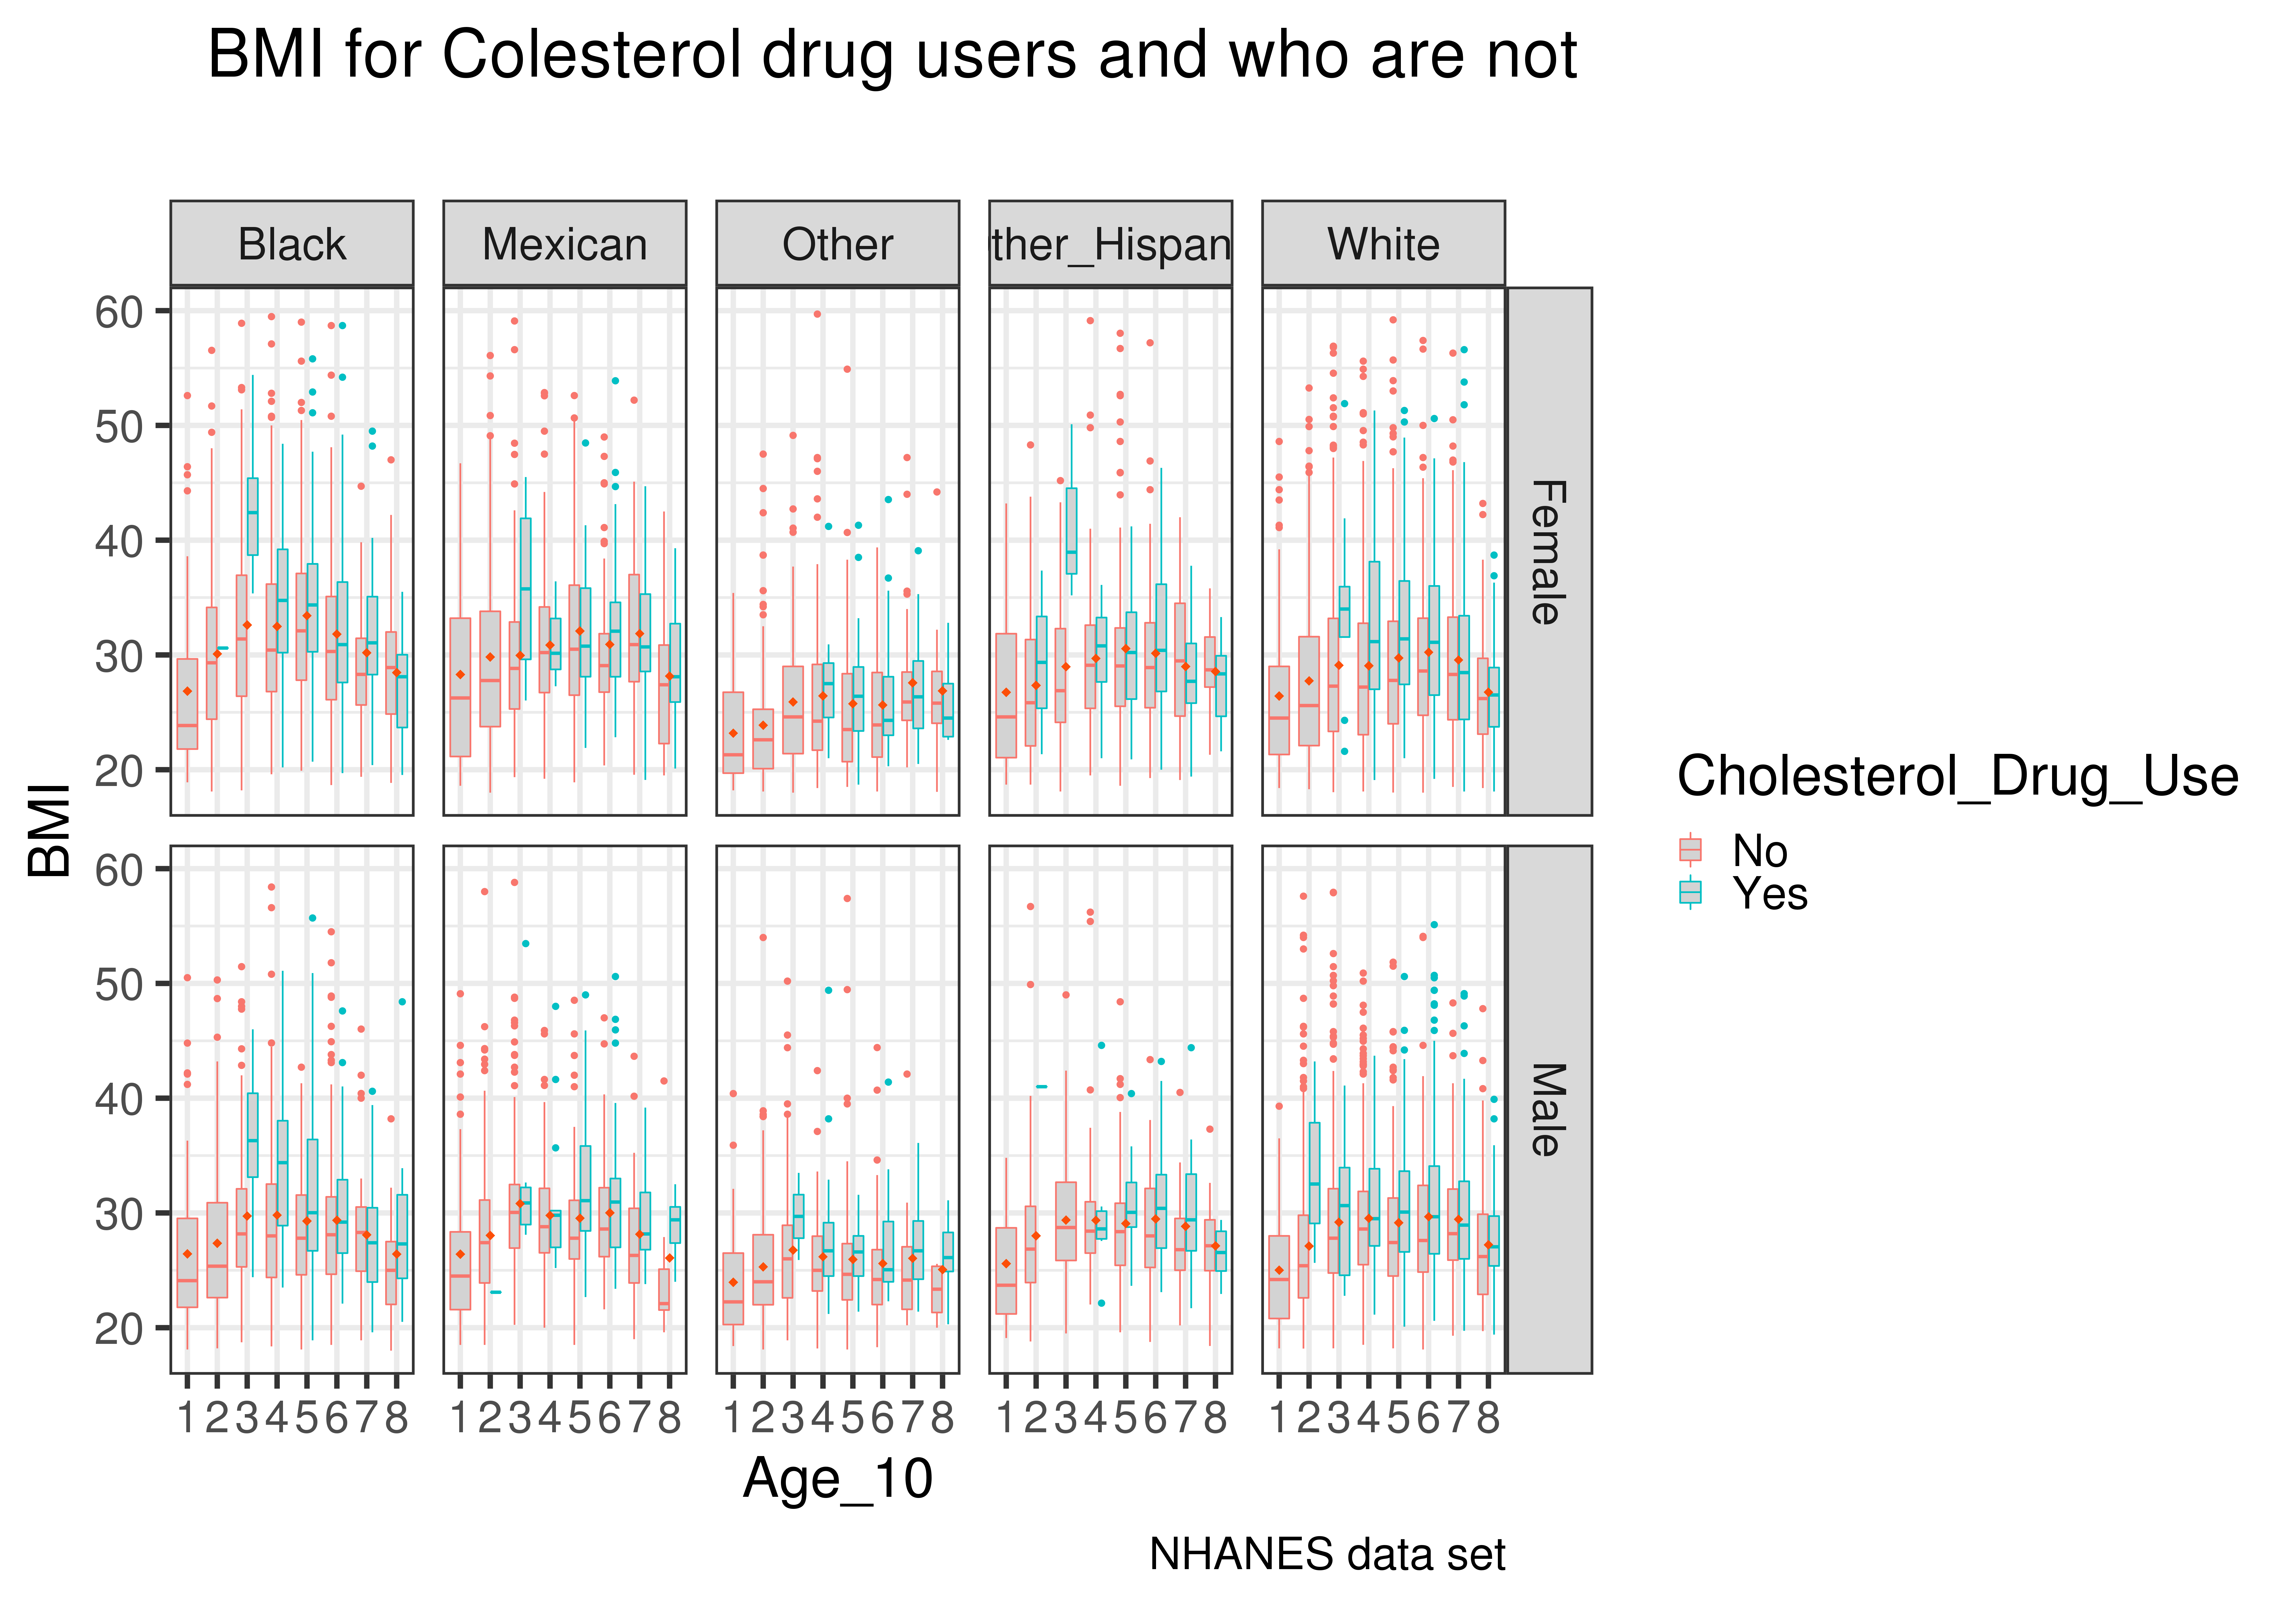
\includegraphics[width=1\linewidth]{/home/mabdulsa/BMI/images/base_box_plot} 

}

\caption{Illustration of data distribution using a box plot. The plot compares cholesterol medicated users vs non-cholesterol medicated users}\label{fig:box}
\end{figure}

Figure \ref{fig:box} shows how the association between age and BMI given cholesterol medication use changes based on age. At younger ages, the average BMI for black population increases as a function of age up to around age 30 years. For ages more than 40 years, the association becomes negative. This observation suggests that at around 30 year old people start to take care of their weights. Mexican Females do not show significant reduction in the BMI as a function of age. For White Males, the association is flat at the middle ages and negative at older ages. Moreover, at lower ages, cholesterol medications are prescribed only for a population with high varying BMI, but at older ages, the difference in BMI given cholesterol medication status decreases until it diminishes as in the white population. The heterogeneity can also be seen in gender, for the Hispanic female population, the cholesterol medication is taken by the population with lower BMI if compared to the population that does not take cholesterol medication.

\begin{figure}

{\centering 
\includegraphics[width=0.8\linewidth]{/home/mabdulsa/BMI/images/quant90} 

}

\caption{A 90th quantile of BMI ploted with repect to age. The population grouped with repect gender and fasting blood glucose level: prediabetes nad diabetes}\label{fig:unnamed-chunk-1}
\end{figure}

\section{Results}

Figures \ref{fig:resu1} and \ref{fig:resu12} illustrate marginal effects of predictors on different quantiles, where in the first plot age and total cholesterol entered the model as quadratic terms while in the second plot, spline basis expansion is used to model age and total cholesterol. First, we look at the differences in the plot that is due to using OLS vs QR, then we look at the differences due to the using quadratic term to model predictors vs spline basis expansion.

From Figures \ref{fig:resu1}, we can see the effects on conditional mean of BMI level may not reflect the size and nature of these effects on lower or upper quantiles. For example, the conditional mean effect of gender on BMI level is about -1 \(kg/m^2\), that is, on average a male BMI is less than female BMI by 1 \(kg/m^2\). However, at the lower quantiles males have higher BMI by 1 \(kg/m^2\). Then, the differences start to diminish up to 0 at 40th quantile. At higher quantiles, a male BMI is less than a female BMI. For example, at 60th quantile a male BMI is less than a female BMI by 1 \(kg/m^2\), and it continue to increase up to 3\(kg/m^2\) at 90th quantile.

From the OLS it is obvious cholesterol medication users have on average higher BMI levels if compared to non-cholesterol medicated users which are around 1.75. The disparity is almost consistent throughout different BMI quantiles. For example, in the lower quantiles of the distribution the cholesterol medicated users have higher BMI value by about 1.5 \(kg/m^2\) on average, but around at 50 th percentile of the conditional distribution the difference is on average 1.8 \(kg/m^2\). Overall, cholesterol medication use seems to be associated with rather large effects on BMI levels somewhat between 1 to 2 \(kg/m^2\) on average.

\begin{figure}

{\centering 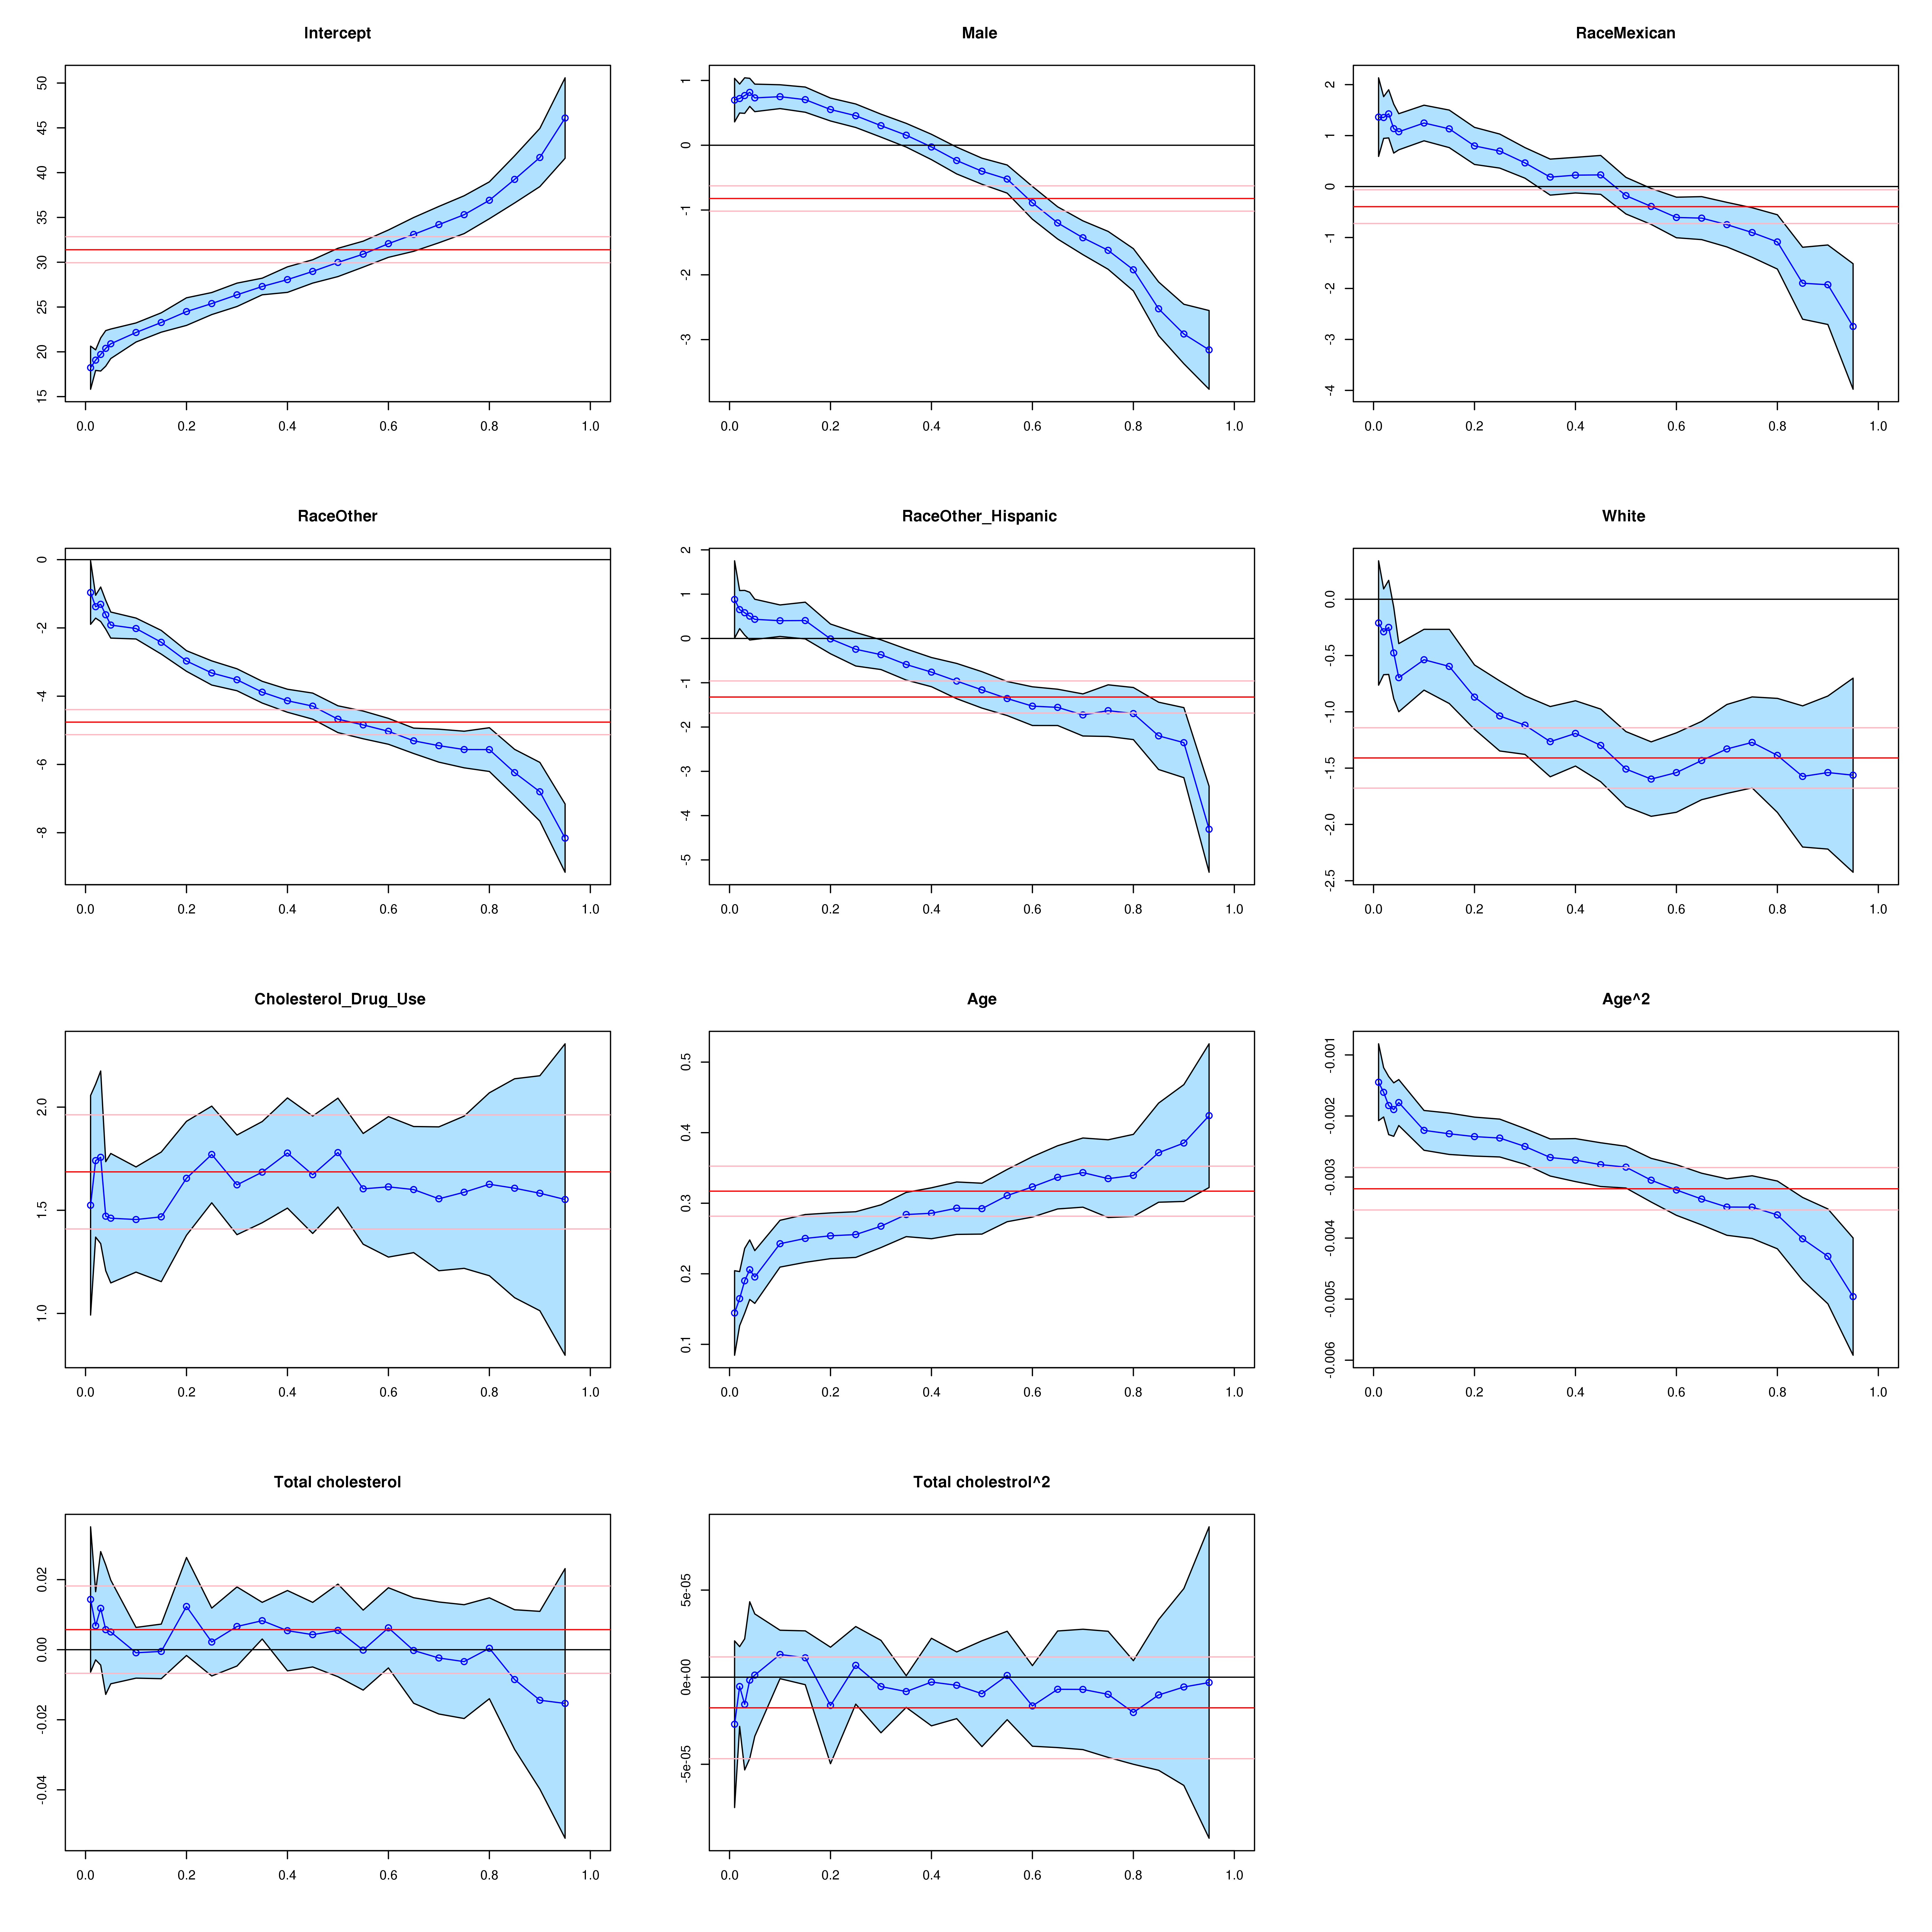
\includegraphics[width=1\linewidth]{/home/mabdulsa/BMI/images/newfig} 

}

\caption{Quantile regression of BMI ploted  for different marginal effects. The predictors modeled using quadratic terms. }\label{fig:resu1}
\end{figure}

\begin{figure}

{\centering 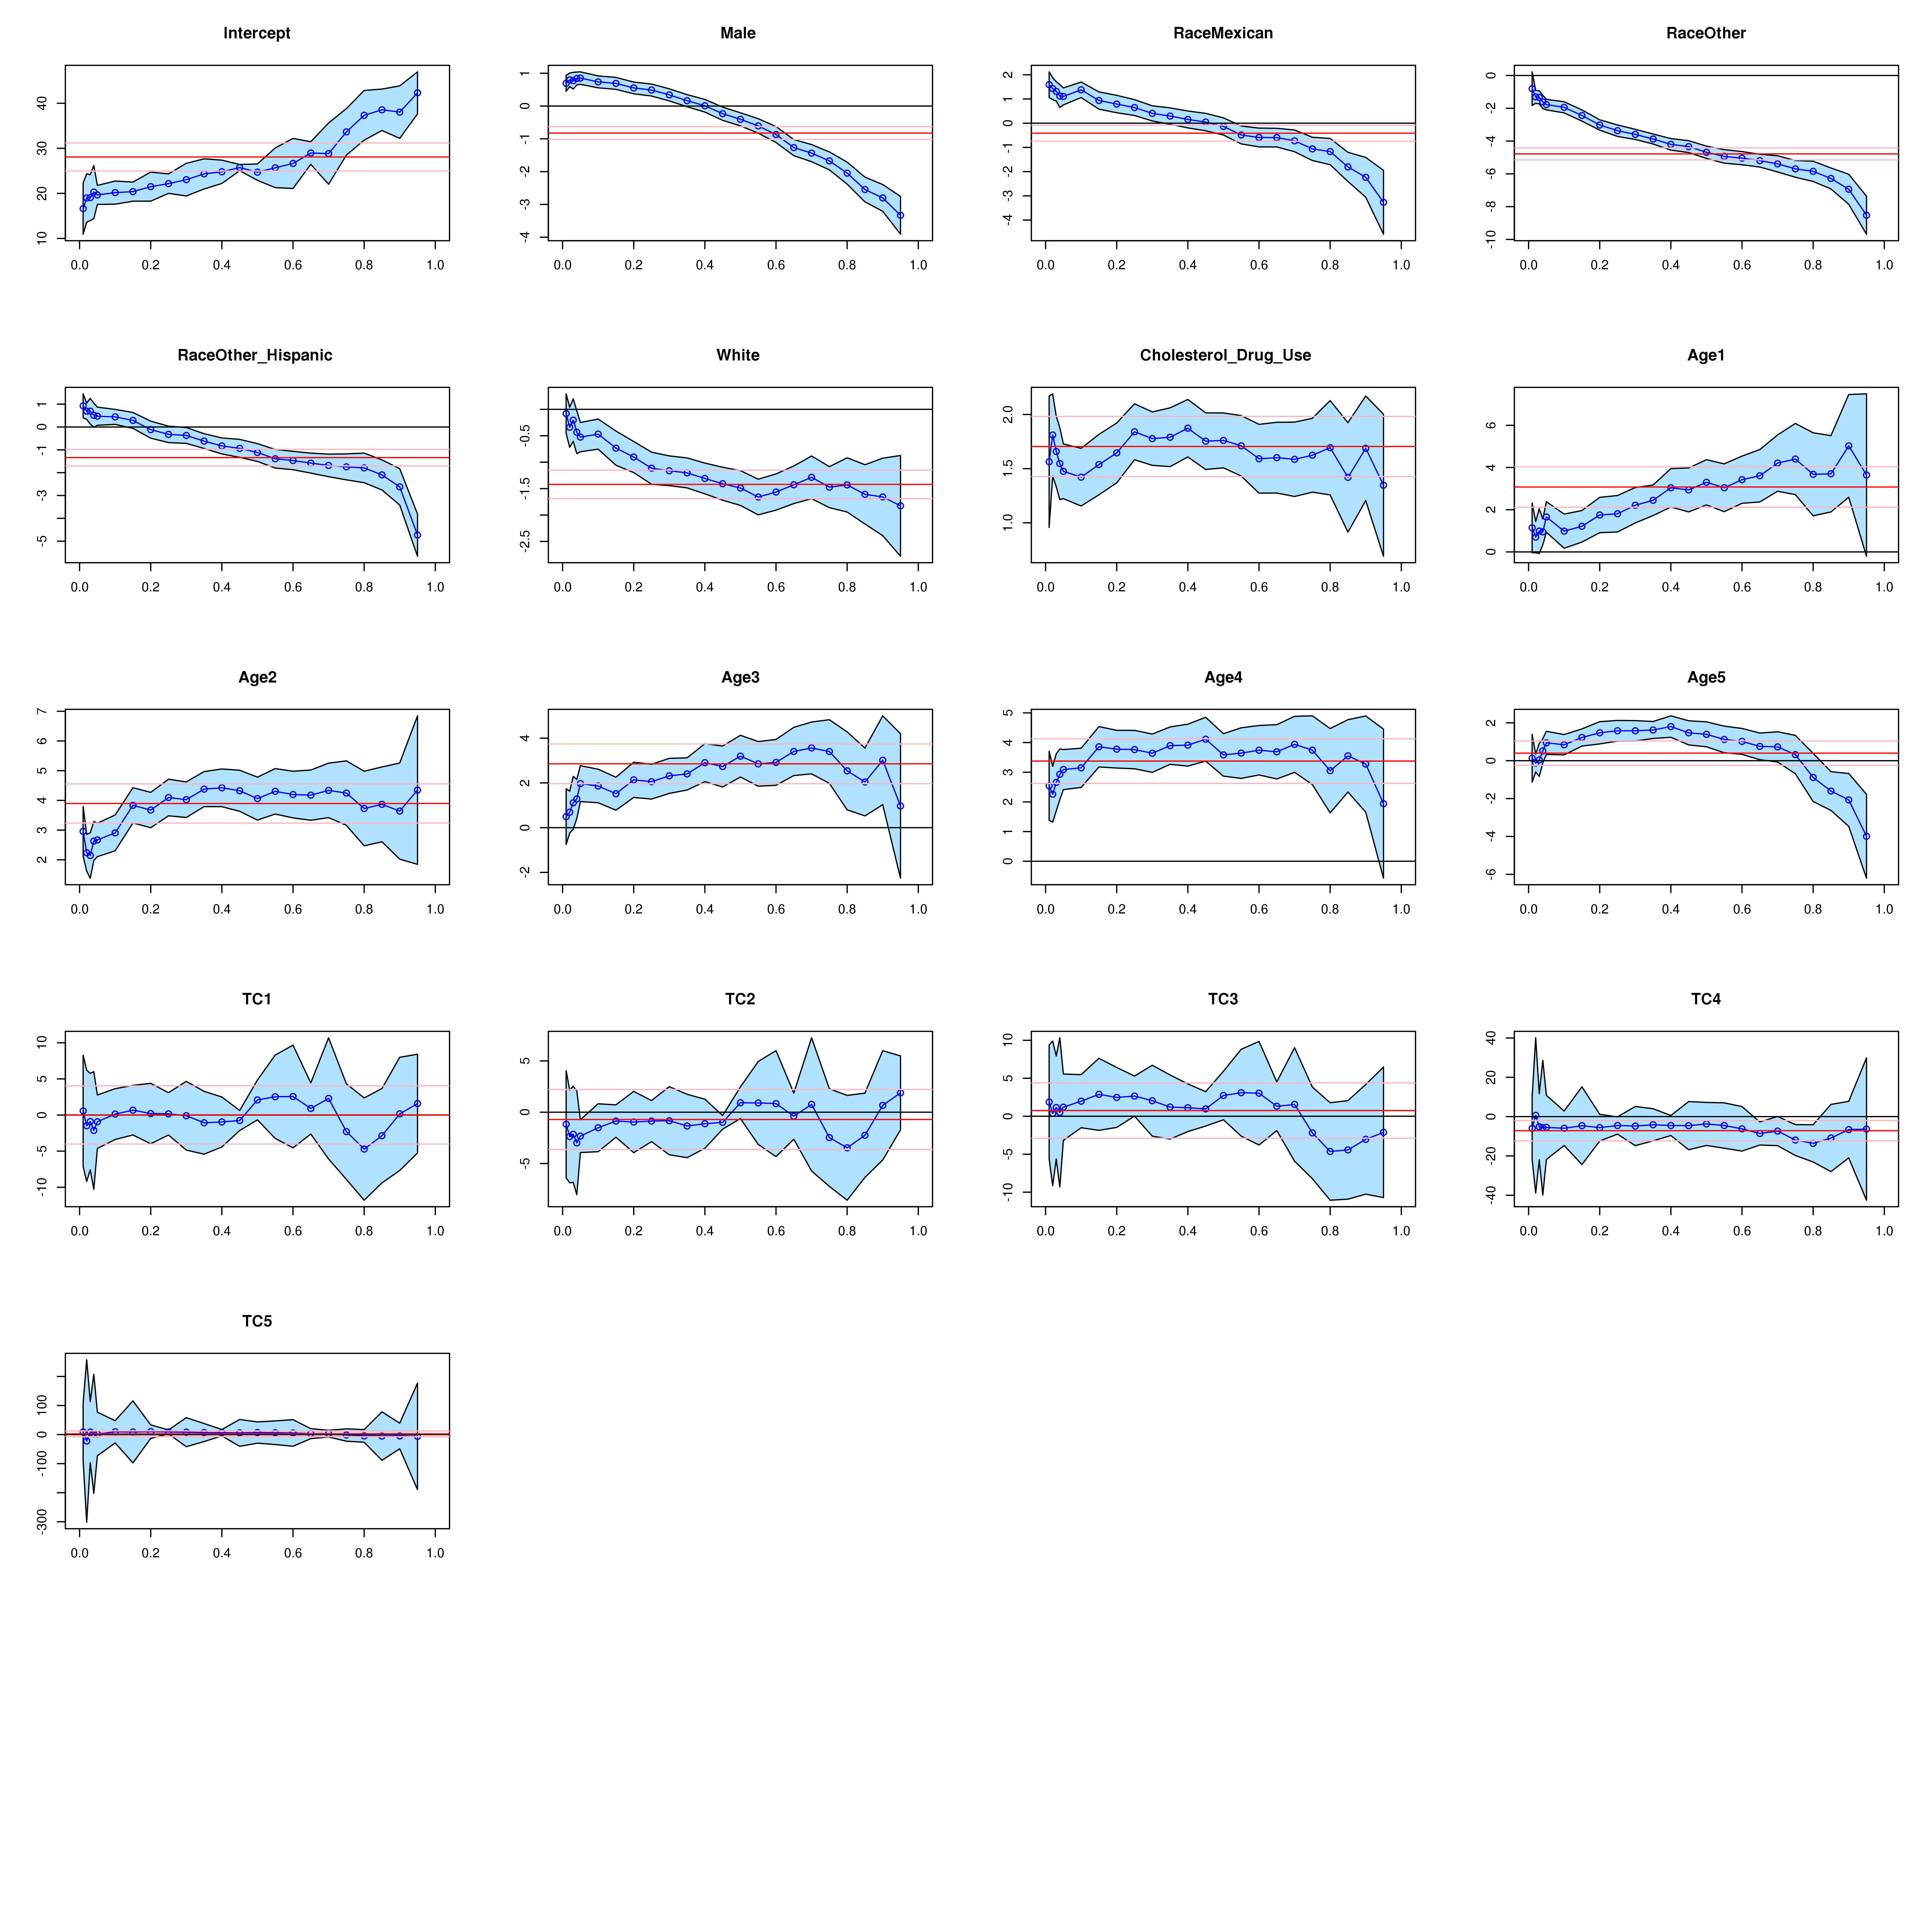
\includegraphics[width=1\linewidth]{/home/mabdulsa/BMI/images/newfig11} 

}

\caption{Quantile regression of BMI ploted  for different marginal effects. The predictors modeled using splines. }\label{fig:resu12}
\end{figure}

\subsection{Age effects Analysis}

Figure \ref{fig:resu1000} illustrate the differences in modeling age in two different ways (Model III; spline basis expansion) and (Model I; quadratic term ).\\
Model III shows, at the lower quantile, the marginal age effects on BMI increases from age 20 to around age 42, and then it stays flat up to age 70 but it starts to decrease after that. While model I shows that there is positive relationship between Age and BMI in the age range between 20 and 50. Then age effects stay flat in the age range between 50 and 60 years old and decreases after that.

At the 50th quantile, model III shows the highest age effect on BMI occurs earlier by 10 years when compares to the lower quantile, but model I shows maximum effect occurs at around age 50, which is similar to the age effect at lower quantiles. The age effects start to decrease using Model III at around 70 years old while model I shows the decay starts at around age 60.\\
At higher quantiles (\(\tau=75\)) Model III shows the maximum age effects occurs at age around 32 years old, which is earlier than the age at which the peak coccurs in by three years than , but Model I shows the highest age effects occurs at around age 50. The decay, according to Model III, starts at around age 70 years old, but Model I shows the decay starts earlier at around 70 years old. Convex behavior of the quadratic term has a clear pattern in formulating age effects on the BMI. The box plot (Fig. \ref{fig:box}) supports Model III results because the highest mean and inter quantile range occurs at age 30.

Using Model III, at the 90th quantile of the conditional BMI distribution, we have a similar behavior as in 0.75th quantile except the relationship is stronger, i.e, for example, the age effects at age 20 is 37 \(kg/m^2\) while at the later the effect is 30 \(kg/m^2\). The BMI trend in this modeling is close to the trend shown in (Chen 2005), which computed using a complicated polynomial and log transformation for the response. Our conclusion from Figure \ref{fig:resu1000} is that the marginal age effects on BMI is different on different quantiles. Moreover, modeling age as quadratic term or as spline basis expansion produce different effect with respect to different quantiles of the conditional BMI distribution.

\begin{figure}

{\centering 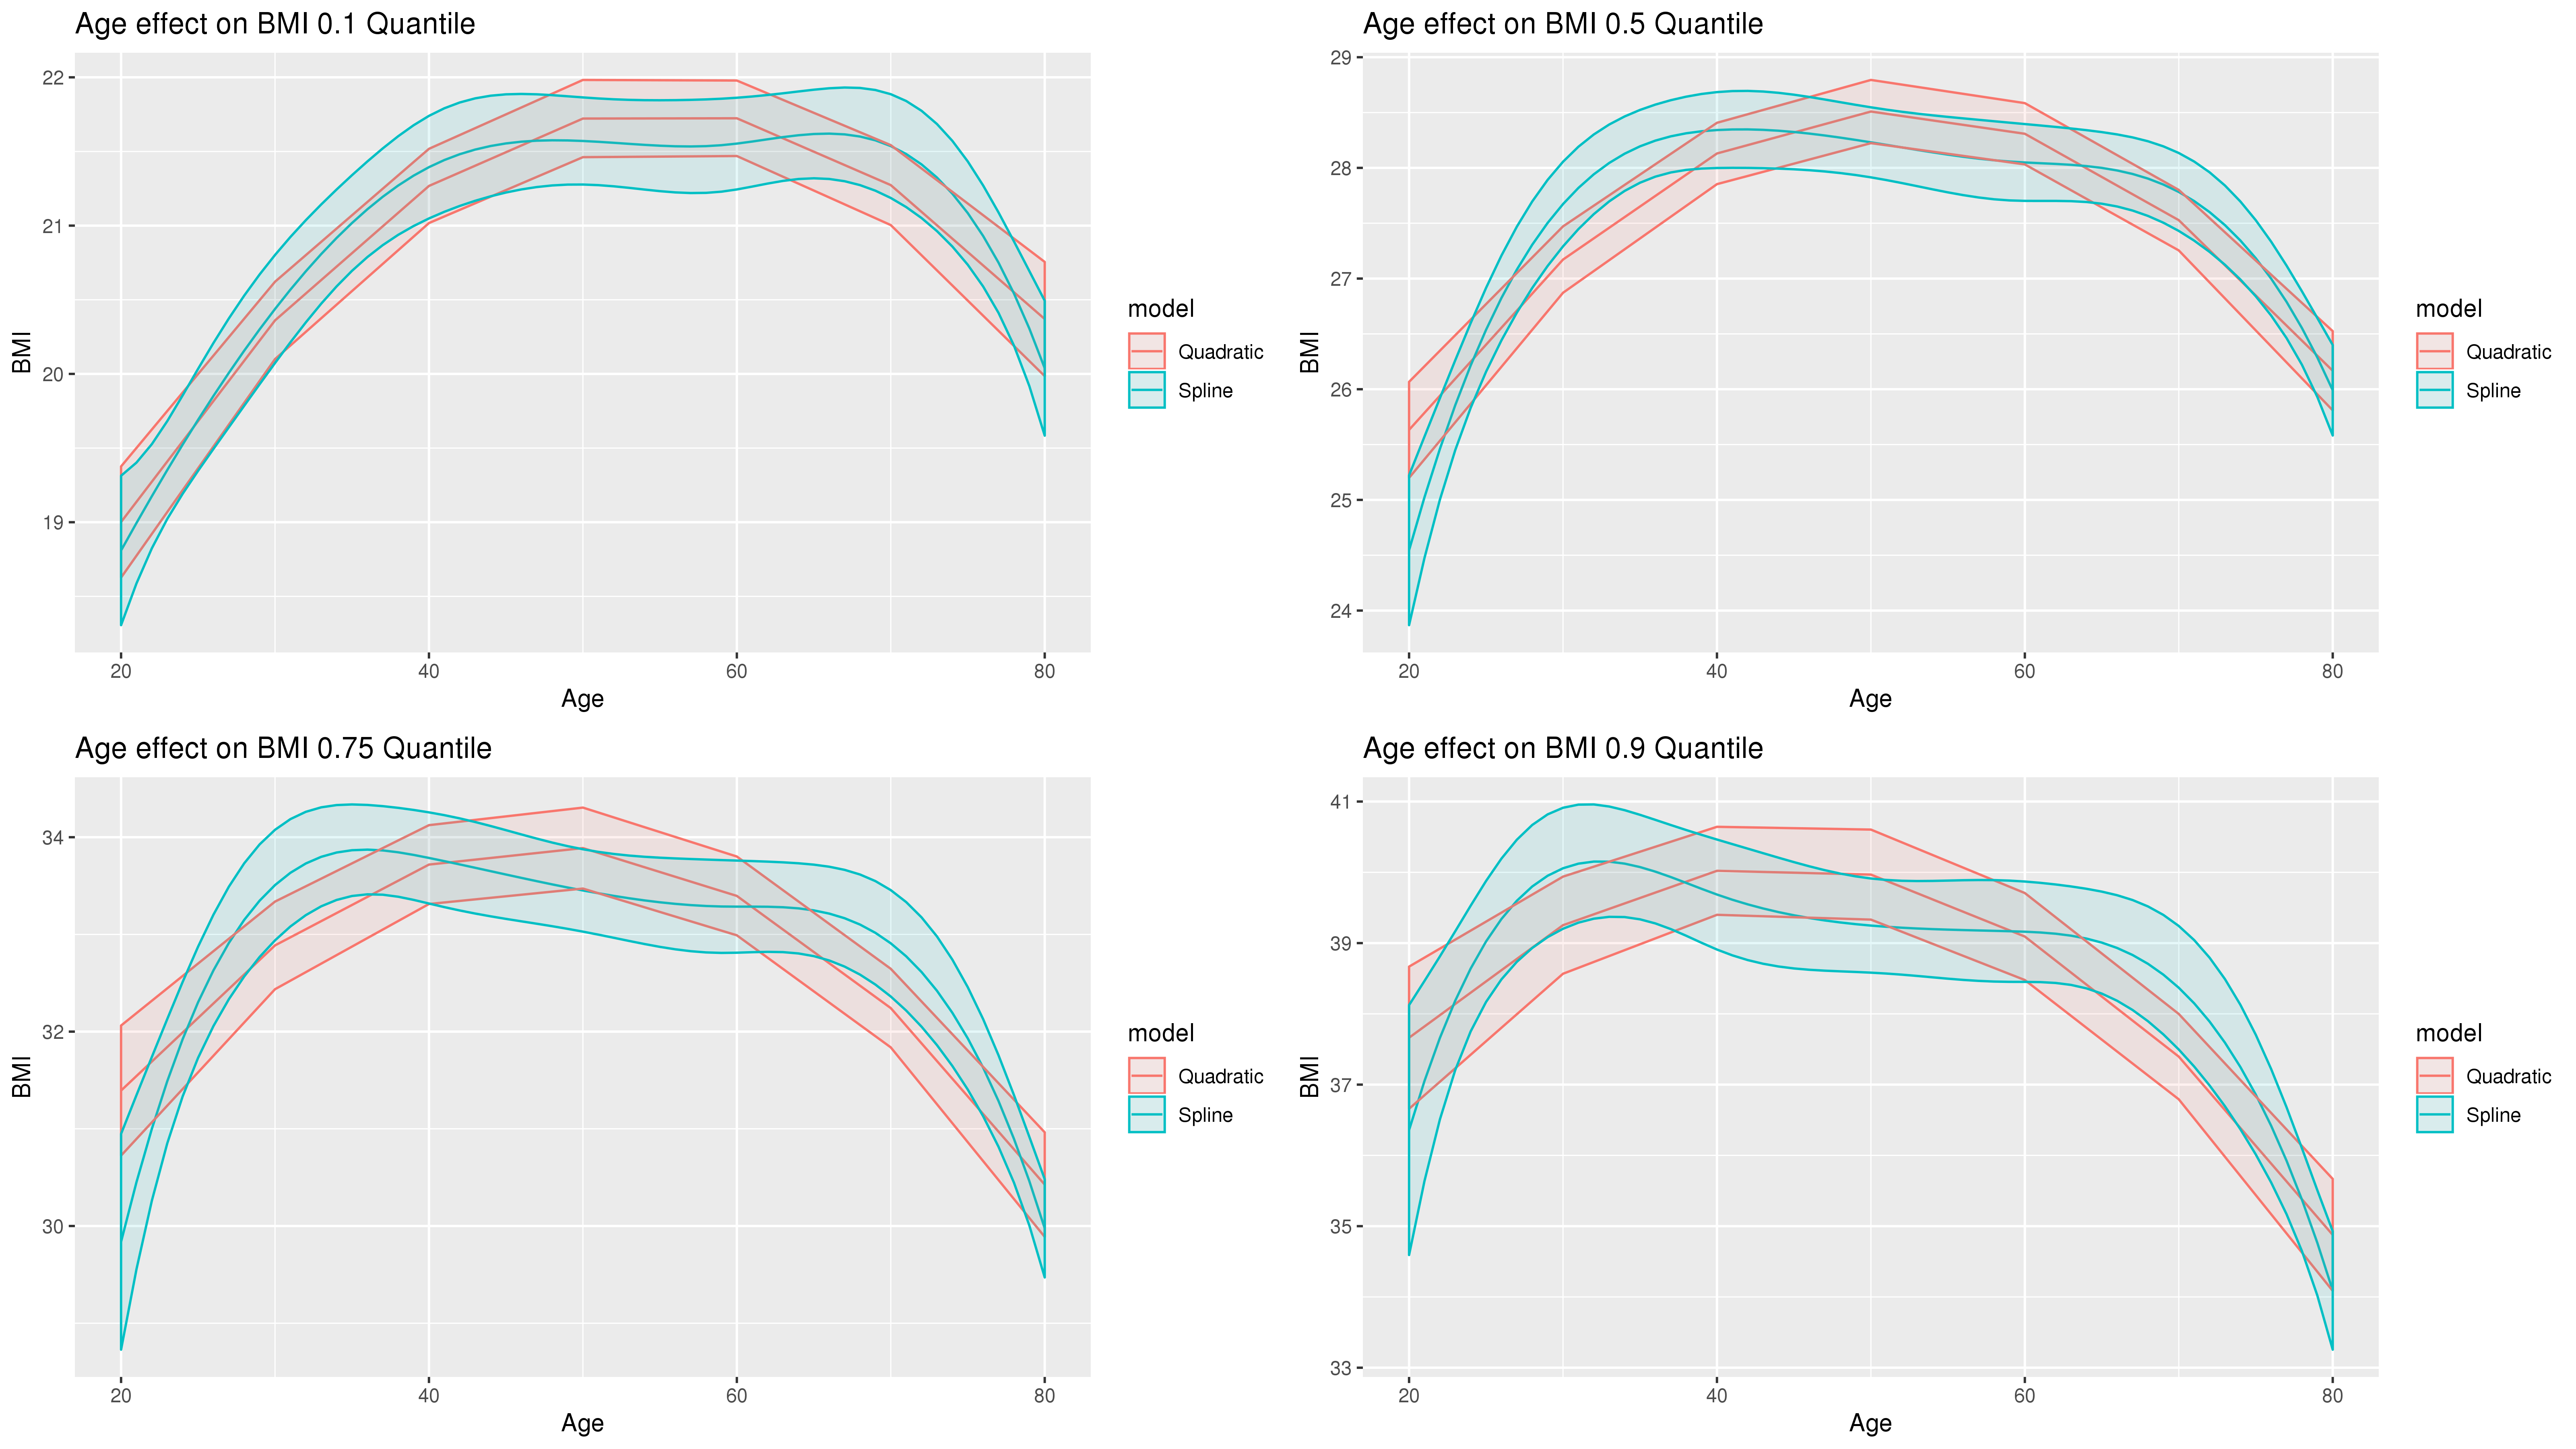
\includegraphics[width=1\linewidth]{/home/mabdulsa/BMI/images/comp_age_mixed} 

}

\caption{  An illustration for the differences in modeling the age effects on different BMI quantiles. The predictors (Age) modeled using quadratic terms and basis splines expension.}\label{fig:resu1000}
\end{figure}
\subsection{TC effects Analysis}

Figure \ref{fig:resu1010} presents the marginal effect of TC for four different quantiles of the conditional distribution of the BMI.
The quadratic effect of total cholesterol on the conditional distribution of BMI is required to be convex when age is modeled using quadratic term. However, TC effect on the BMI is different when TC is modeled using spline basis expansion. The disparity is due to the same reason mentioned earlier, which is as
TC\(\rightarrow\pm\infty,\) BMI\(\rightarrow \pm\infty).\) At the lower tail (\(\tau=0.1\)), for TC less than 300 mg\(\setminus\)dl, we have positive association, that is, when TC increases, the BMI increases also, on average. Moreover, when TC passes 300 mg\(\setminus\)dl level, spline basis expansion modeling of TC presents negative correlation between TC and BMI while quadratic modeling of TC shows positive correlation. In addition, the confidence interval (CI) for quadratic modeling of age is larger than the CI for spline basis expansion modeling for the age. The CI for quadratic modeling of the age indicate poor fitting while spline basis expansion perform better.

At the 50th quantile of BMI, the two methods of modeling TC shows almost the same trend through whole TC range.\\
At higher quantiles \((\tau=75)\), for TC values less than 350 mg/dL, the association is negative that is as TC cholesterol level increases the BMI decreases, for both functional form for modeling TC. However, the two models differ after TC values passes 350 mg/dL because quadratic functional form forces the TC effect to take a convex shape.
At a higher quantile \((\tau=90),\) both the models for TC show BMI taking a convex shape, but quadratic way of modeling BMI is more parabolic than the spline model. When TC passes 380 mg\(\setminus\)dL, the TC model using the spline basis expansion shows the BMI starts to decrease more slowly compared to the quadratic.

\begin{figure}
 
 {\centering 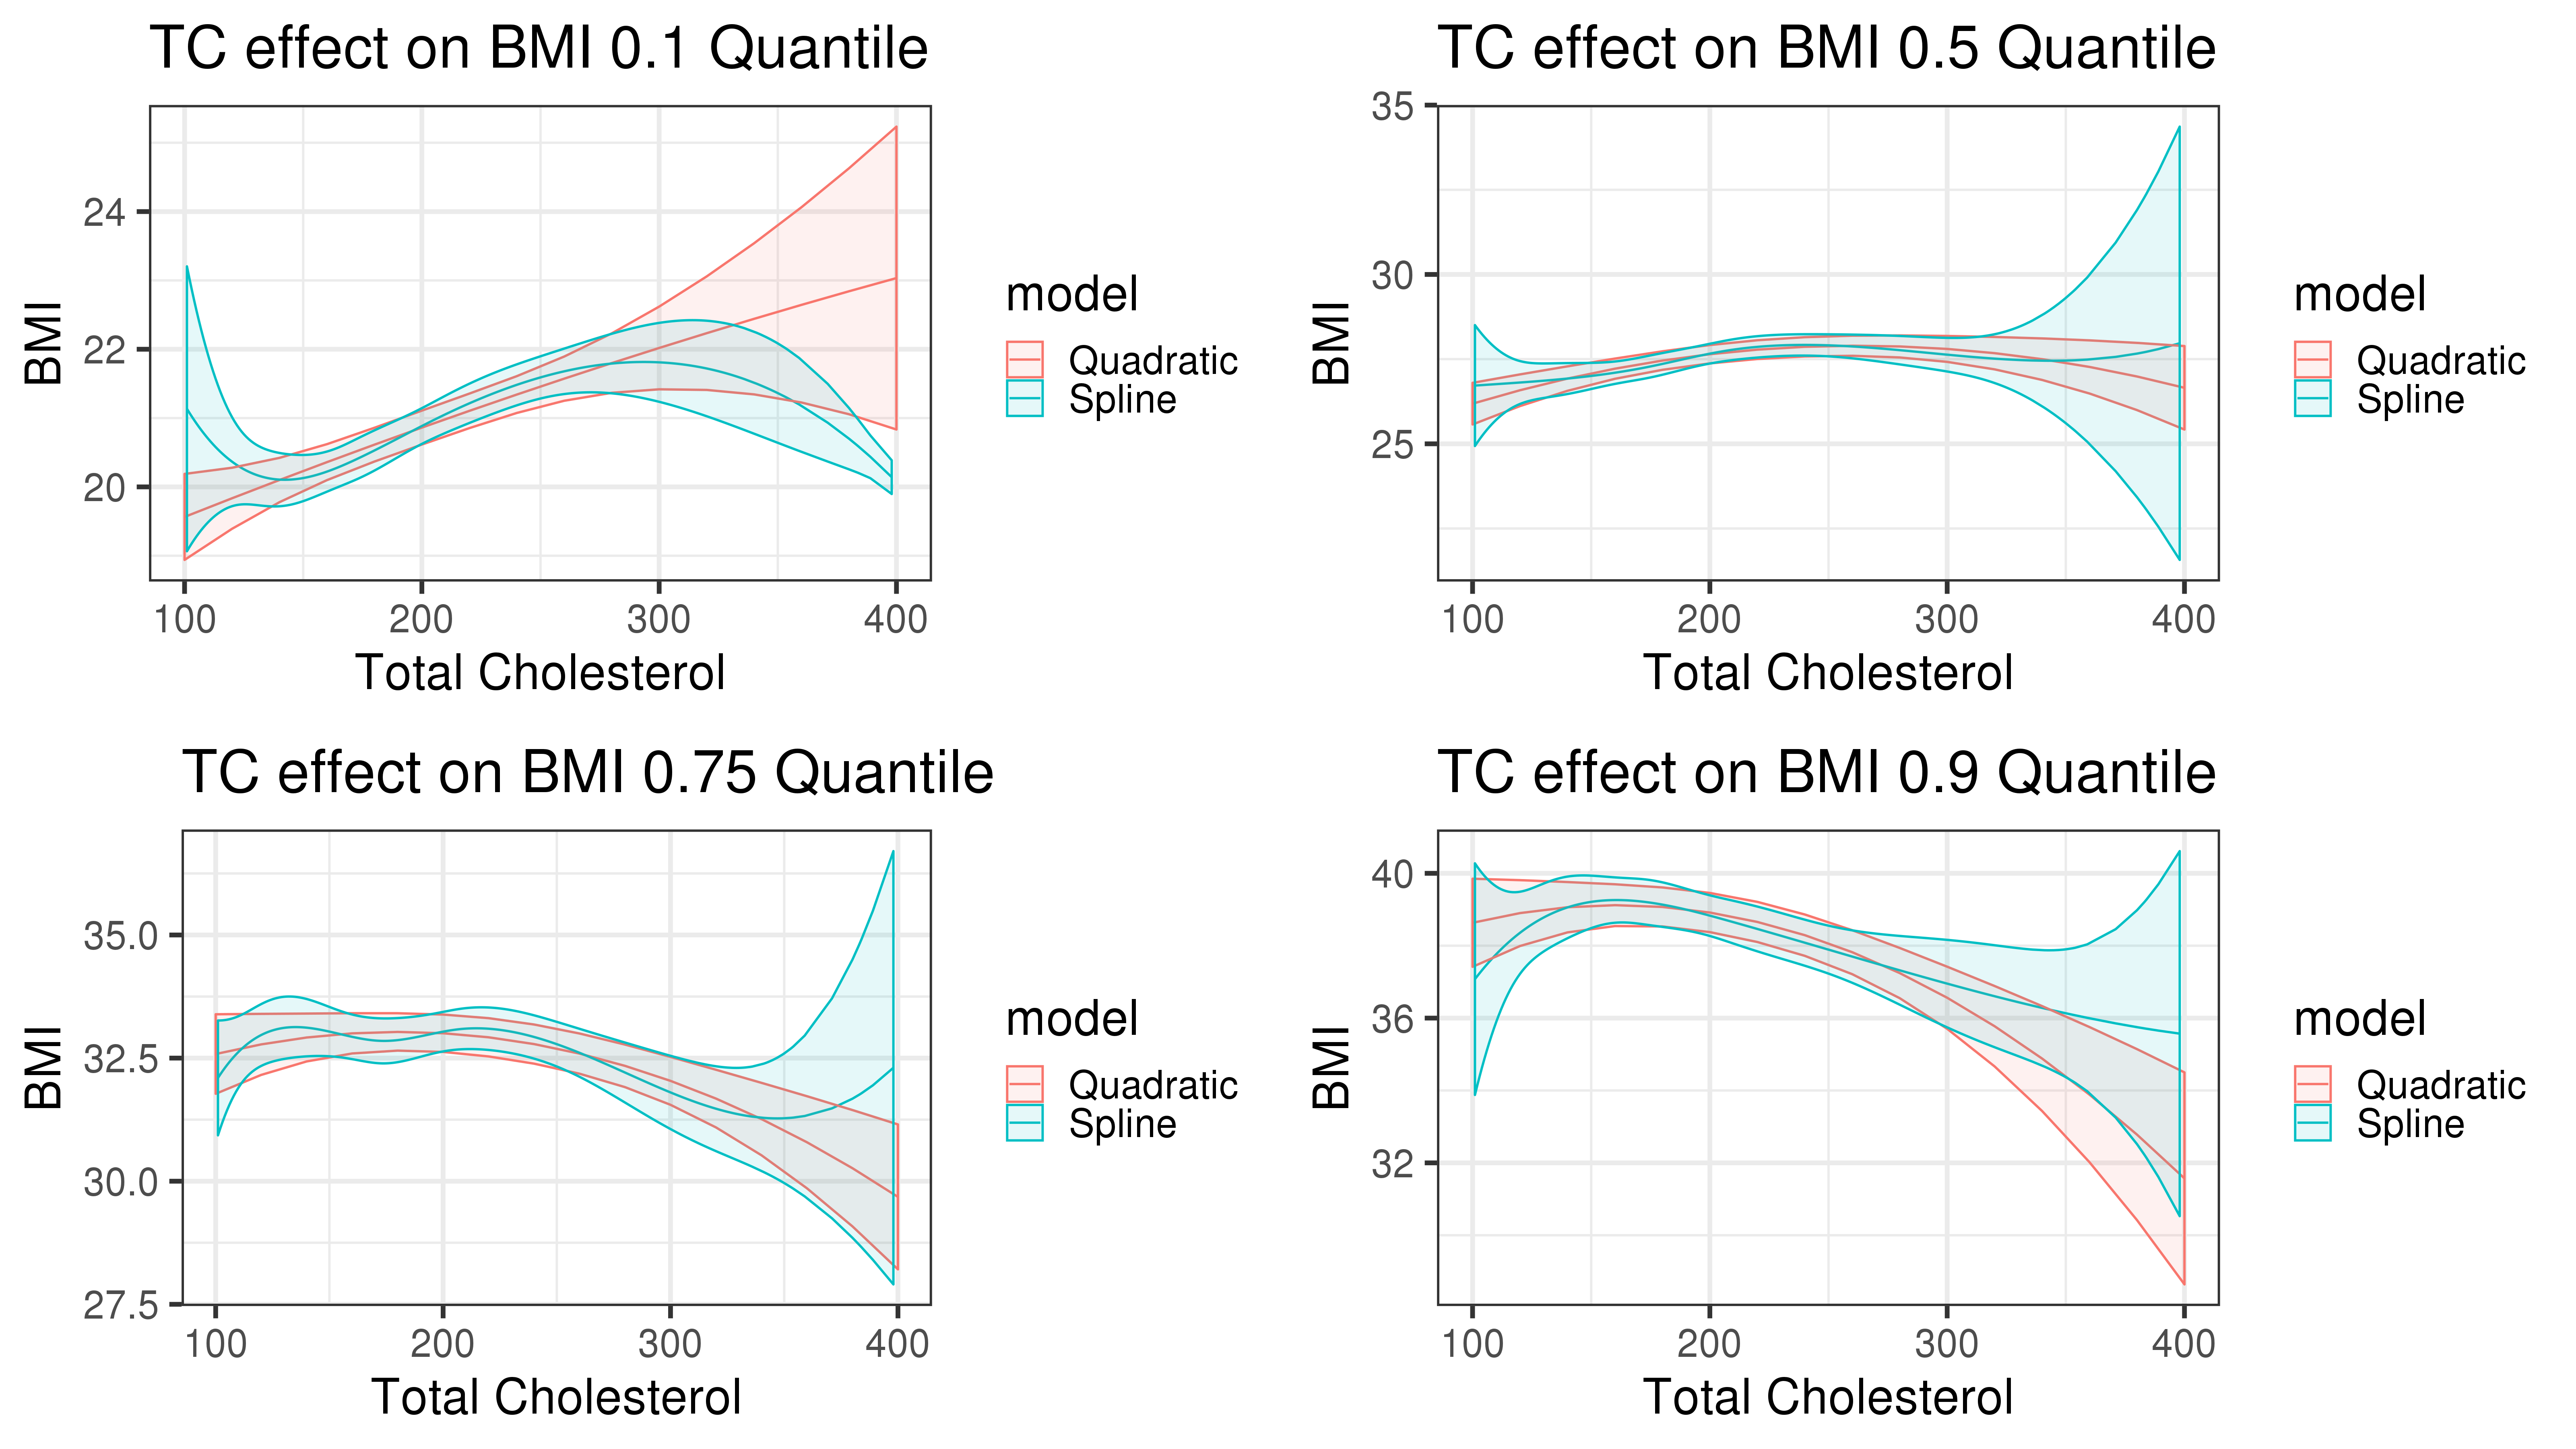
\includegraphics[width=1\linewidth]{/home/mabdulsa/BMI/images/comp_tot_mixed} 
 
 }
 
 \caption{ An illustration of  marginal effects of total cholesterol  on different BMI quantiles. The predictors modeled using quadratic terms and splines. The BMI quantiles $ au=$ 0.1, 0.5, 0.75 and 0.90 coressponds to  21.5,  27.9,  32.4 and 37.7 $kg/m^2$, respectively. }\label{fig:resu1010}
 \end{figure}

For a population with low BMI, it is expected when TC increases (more than 200 mg\(\setminus\)dL), individuals start to reduce their BMI, on average. However, this trend is captured by using spline basis expansion for the TC but it was missed by using quadratic model for TC ( upper left corner plot in Figure \ref{fig:resu1010}.) In addition, an individual with high BMI reduces their weight to reduce their TC. The quadratic modeling of the TC shows a sharp decrease in the BMI when compared to spline basis expansion at \(\tau=0.9\) ( lower right corner of Figure \ref{fig:resu1010}.) As it was shown in (Mc Auley 2020) the obese population has a higher TC and this trend is not captured by quadratic term modeling for TC.

\subsection{Analysing Race/Ethinicity effect on BMI}

Figure \ref{fig:resu3} illustrates age effects on 90th BMI quantile, where age modeled as a quadratic term. There is a clear association between age and BMI. In general, age effects on BMI, considering race ethnicity, behaves at a similar way as the whole population, which is a parabolic shape. For example, a young Mexican female not using cholesterol medication has an average BMI around 40 \(kg/m^2\), but the BMI values decreases later up to 35 \(kg/m^2\) at age 80 years. The effects of age is higher for cholesterol medicated users by an average of about about 2 \(kg/m^2\). Moreover, Mexican males have a higher average BMI than females by about 2 \(kg/m^2\) at \(\tau =0.9\). The lowest age effects on 90th BMI quantile is found in the white race.
In general age effect on BMI for males are higher than for females. Figure \ref{fig:resu33} presents age effect on BMI through using spline basis expansion.

\begin{figure}

{\centering 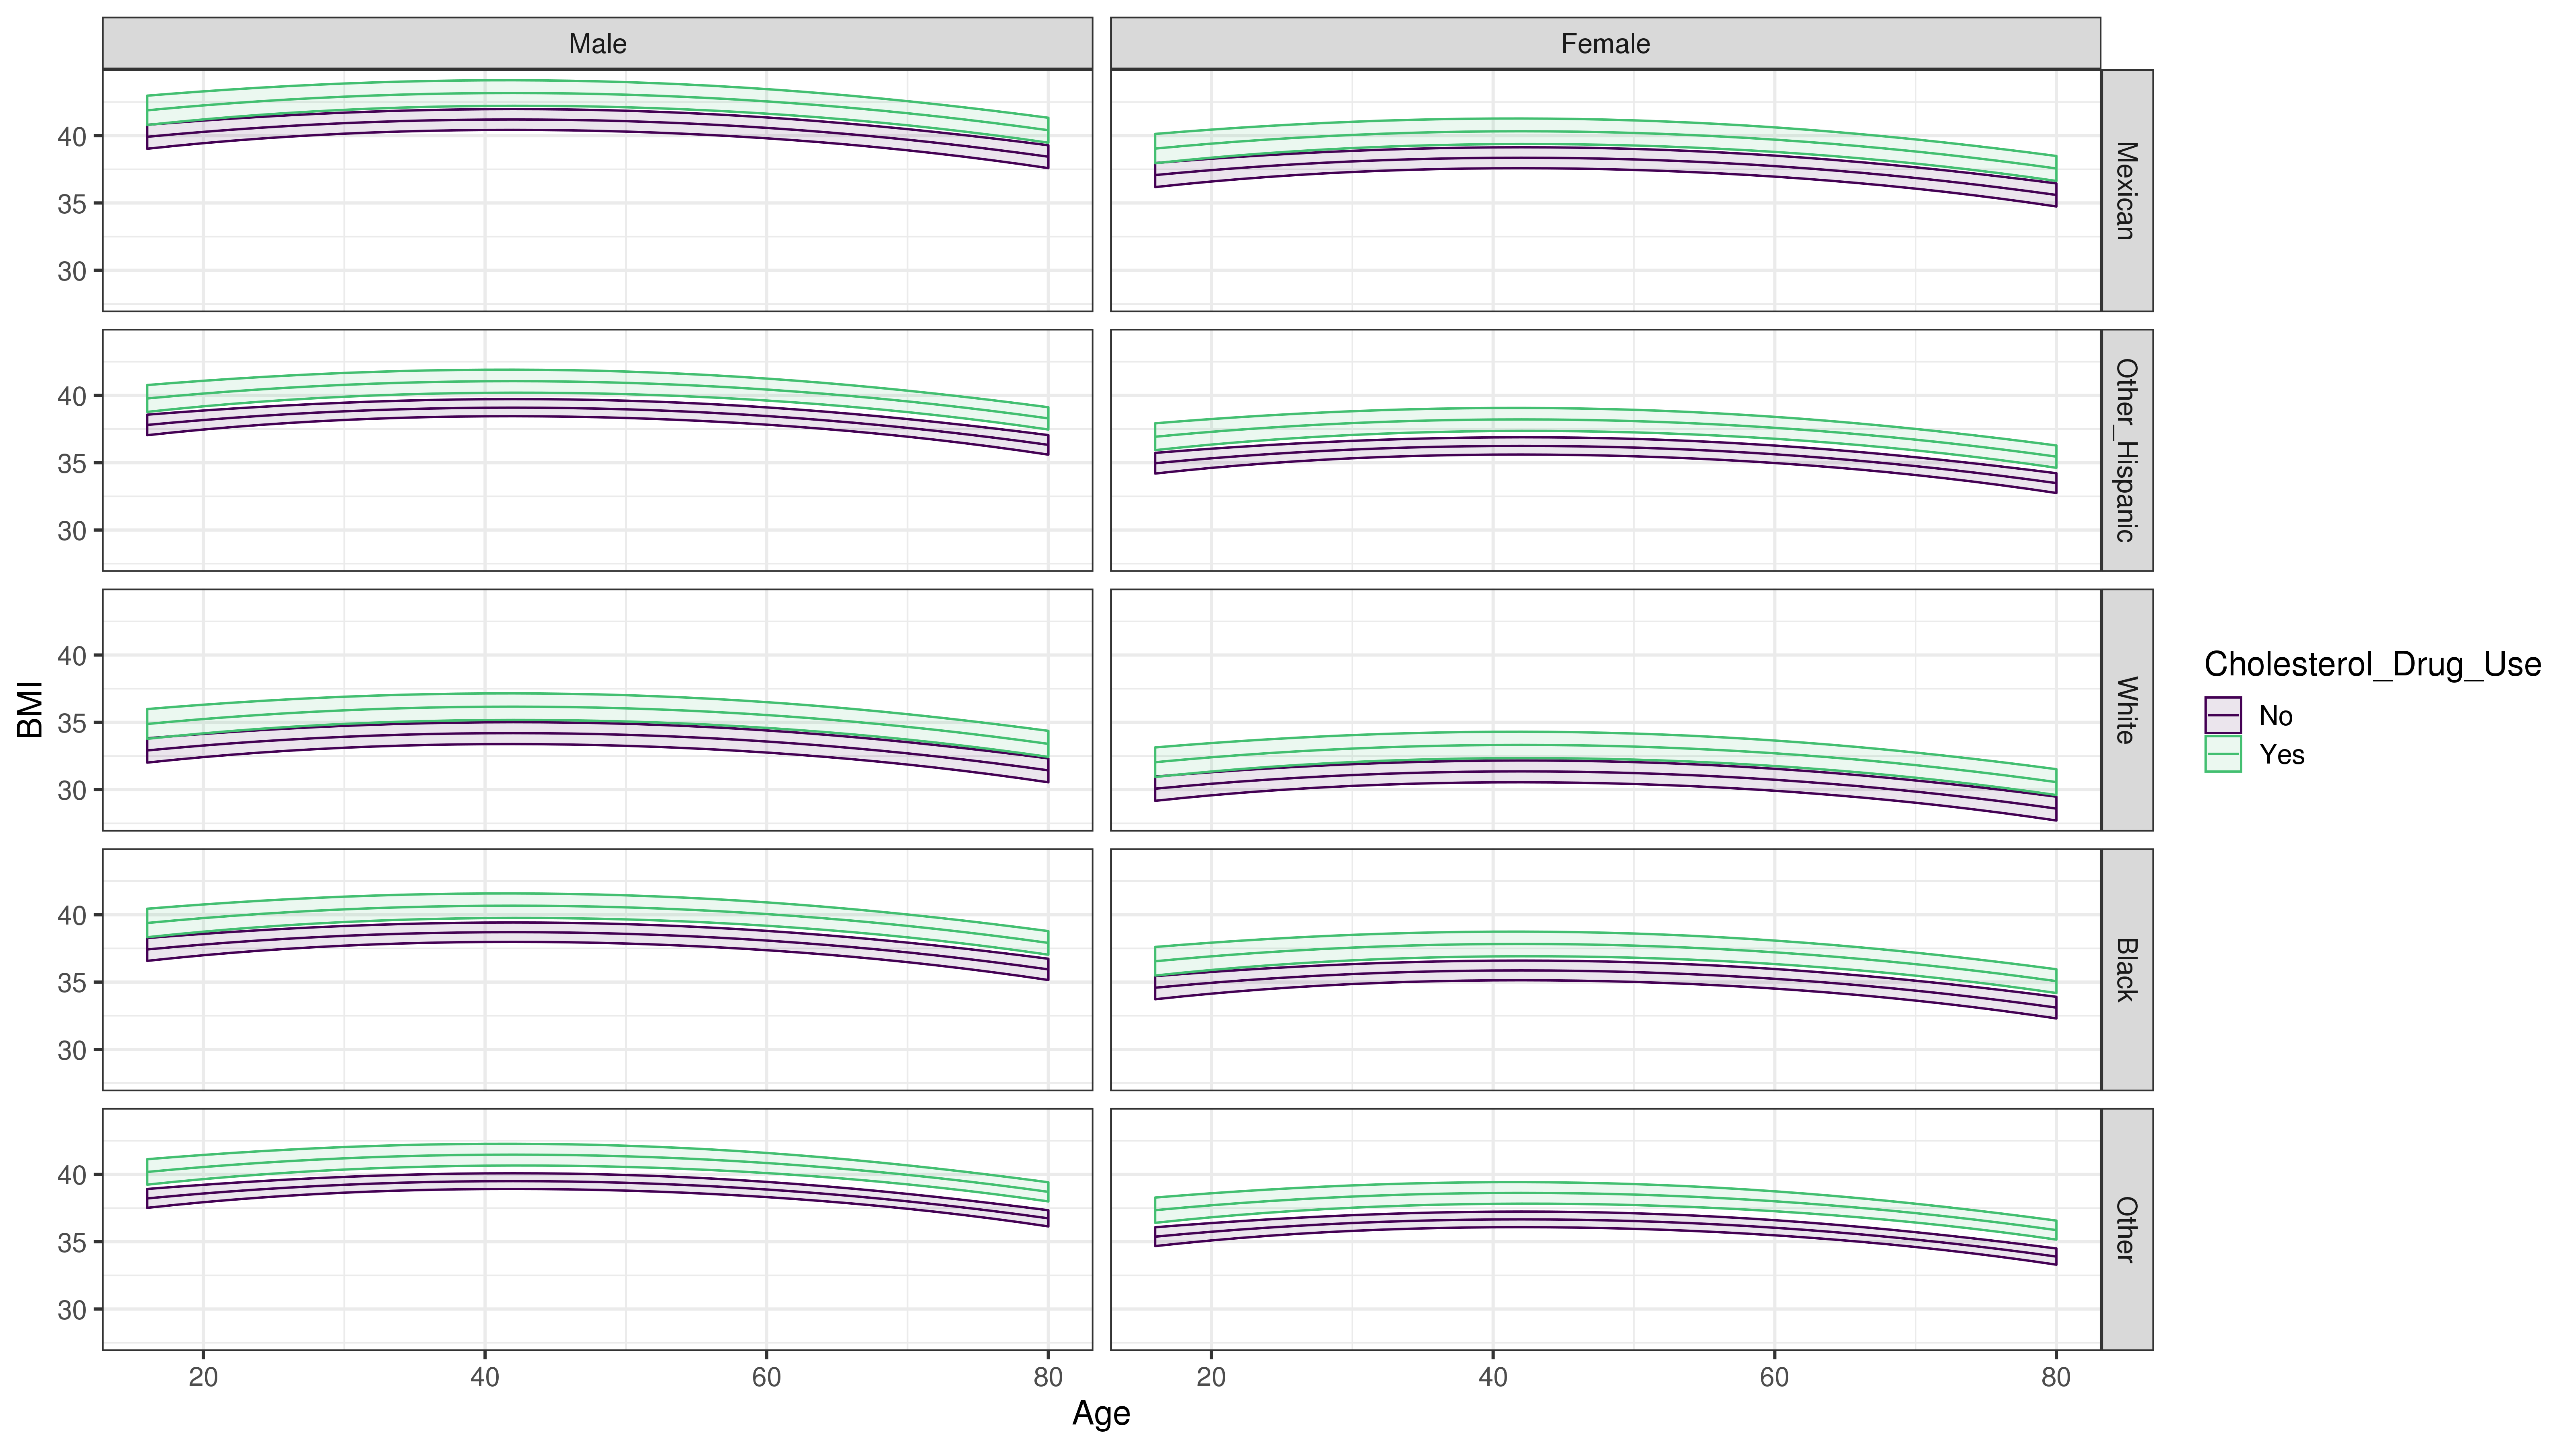
\includegraphics[width=0.8\linewidth]{/home/mabdulsa/BMI/images/Age_poly} 

}

\caption{Illustration of the quadratic age effect on 90th BMI quantile for different race ethnacity groups.}\label{fig:resu3}
\end{figure}

\begin{figure}

{\centering 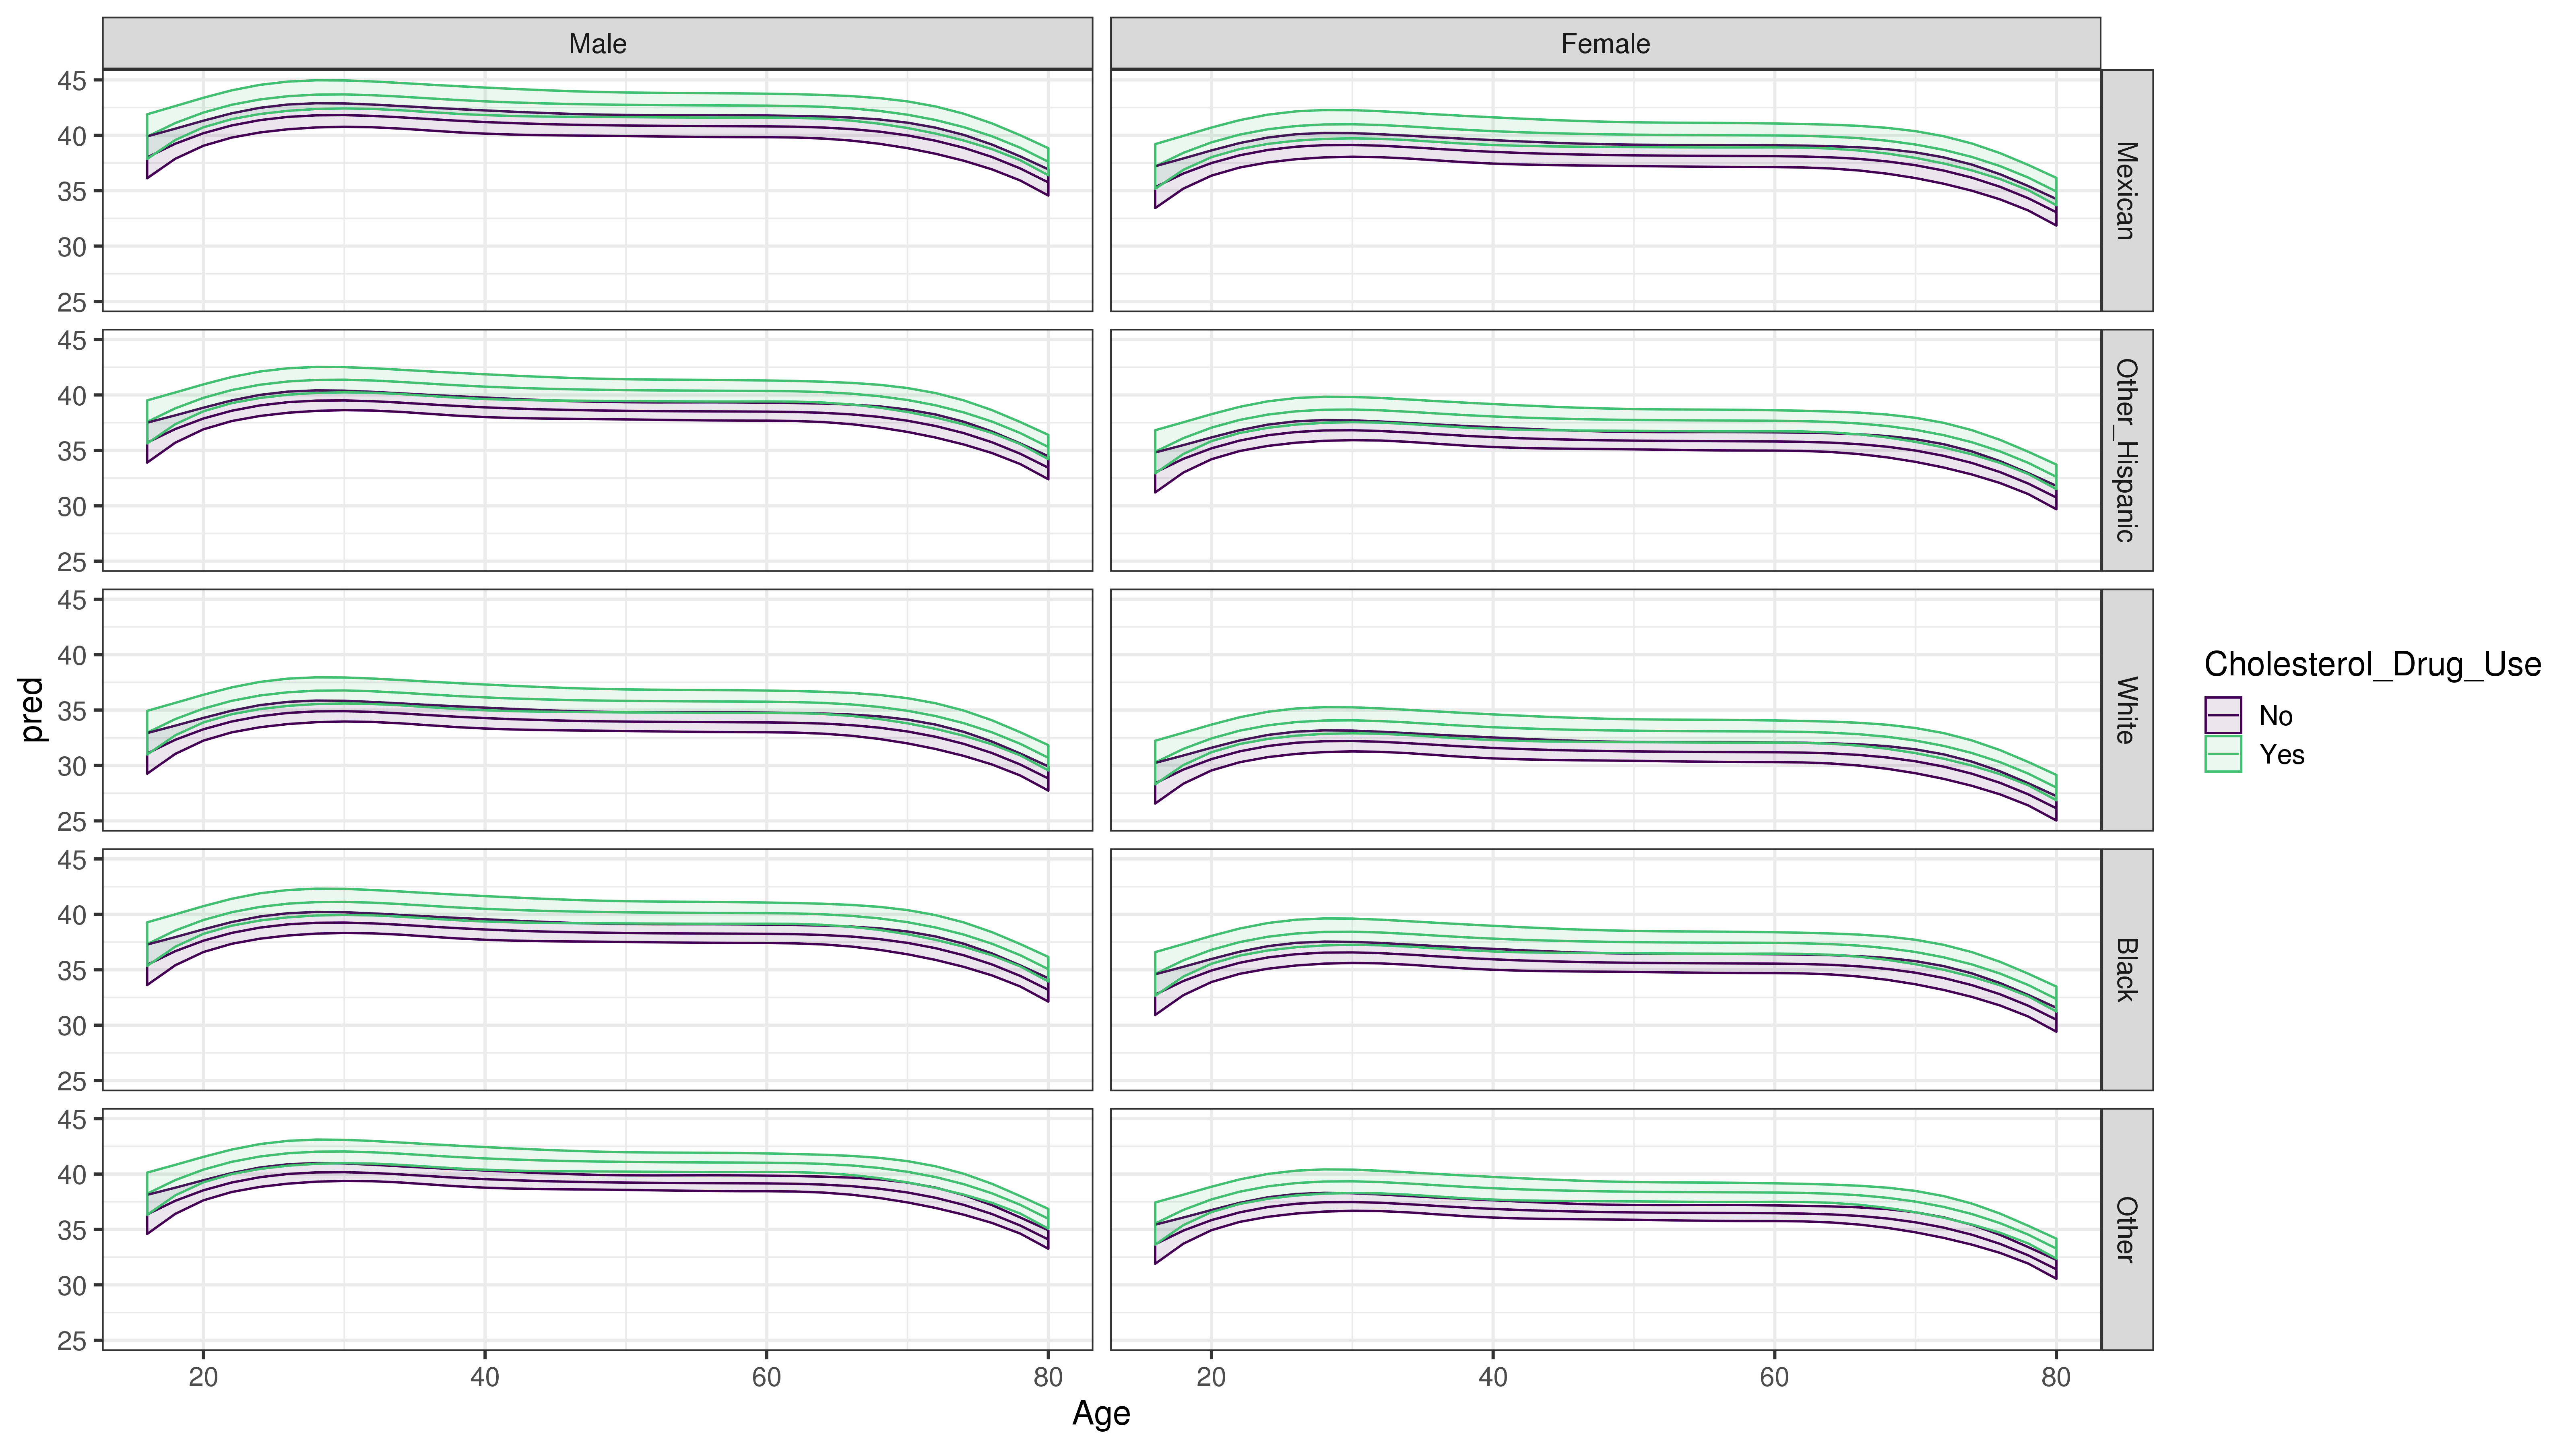
\includegraphics[width=0.8\linewidth]{/home/mabdulsa/BMI/images/Age_splin} 

}

\caption{Illusteration of the age effect on the 90th BMI quantile, where age modeled using spline basis expension. The effect shown for diiferent race/ethenicity groups and gender.}\label{fig:resu33}
\end{figure}

Figure \ref{fig:resu4} and Figure \ref{fig:resu330} present TC effect on BMI with respect to different race/ethnicity groups by modeling TC as a quadratic term and spline basis expansion, respectively. Male population have higher

\begin{figure}

{\centering 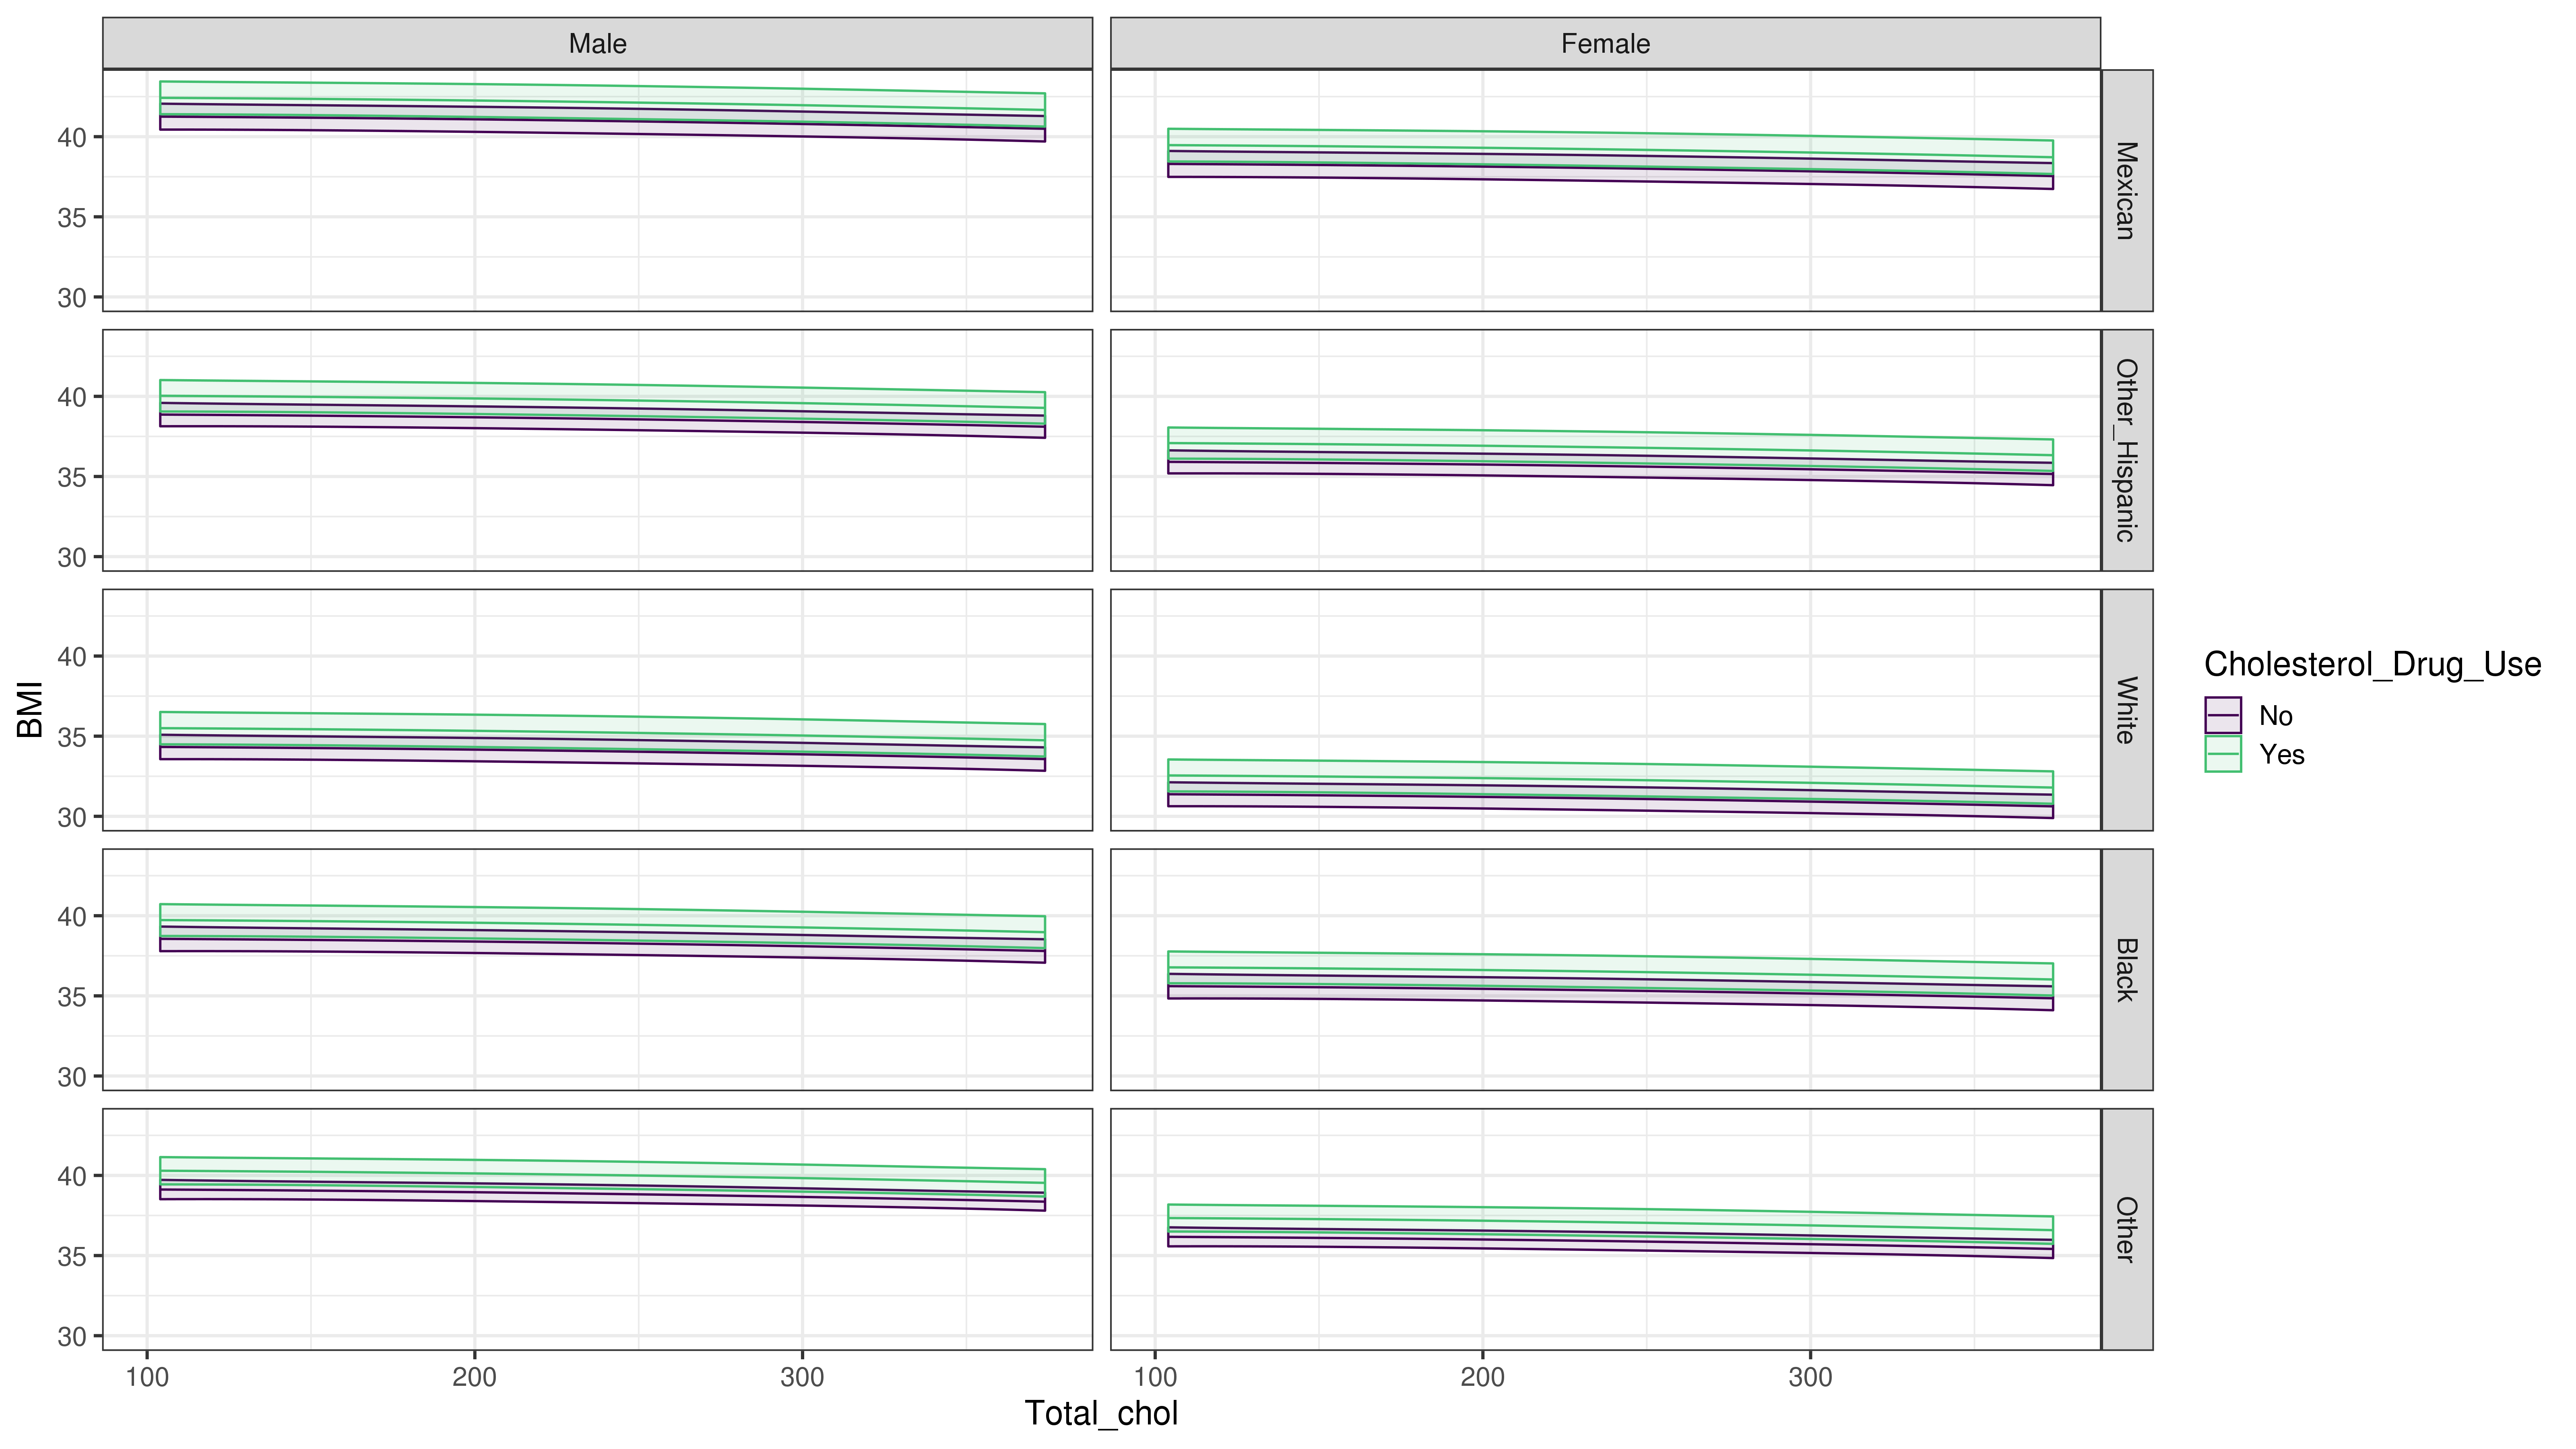
\includegraphics[width=0.8\linewidth]{/home/mabdulsa/BMI/images/Total_chol_poly} 

}

\caption{Illustration of a 90th quantile regression of the BMI. The cholesterol term modeled as  quadratic.}\label{fig:resu4}
\end{figure}

\begin{figure}

{\centering 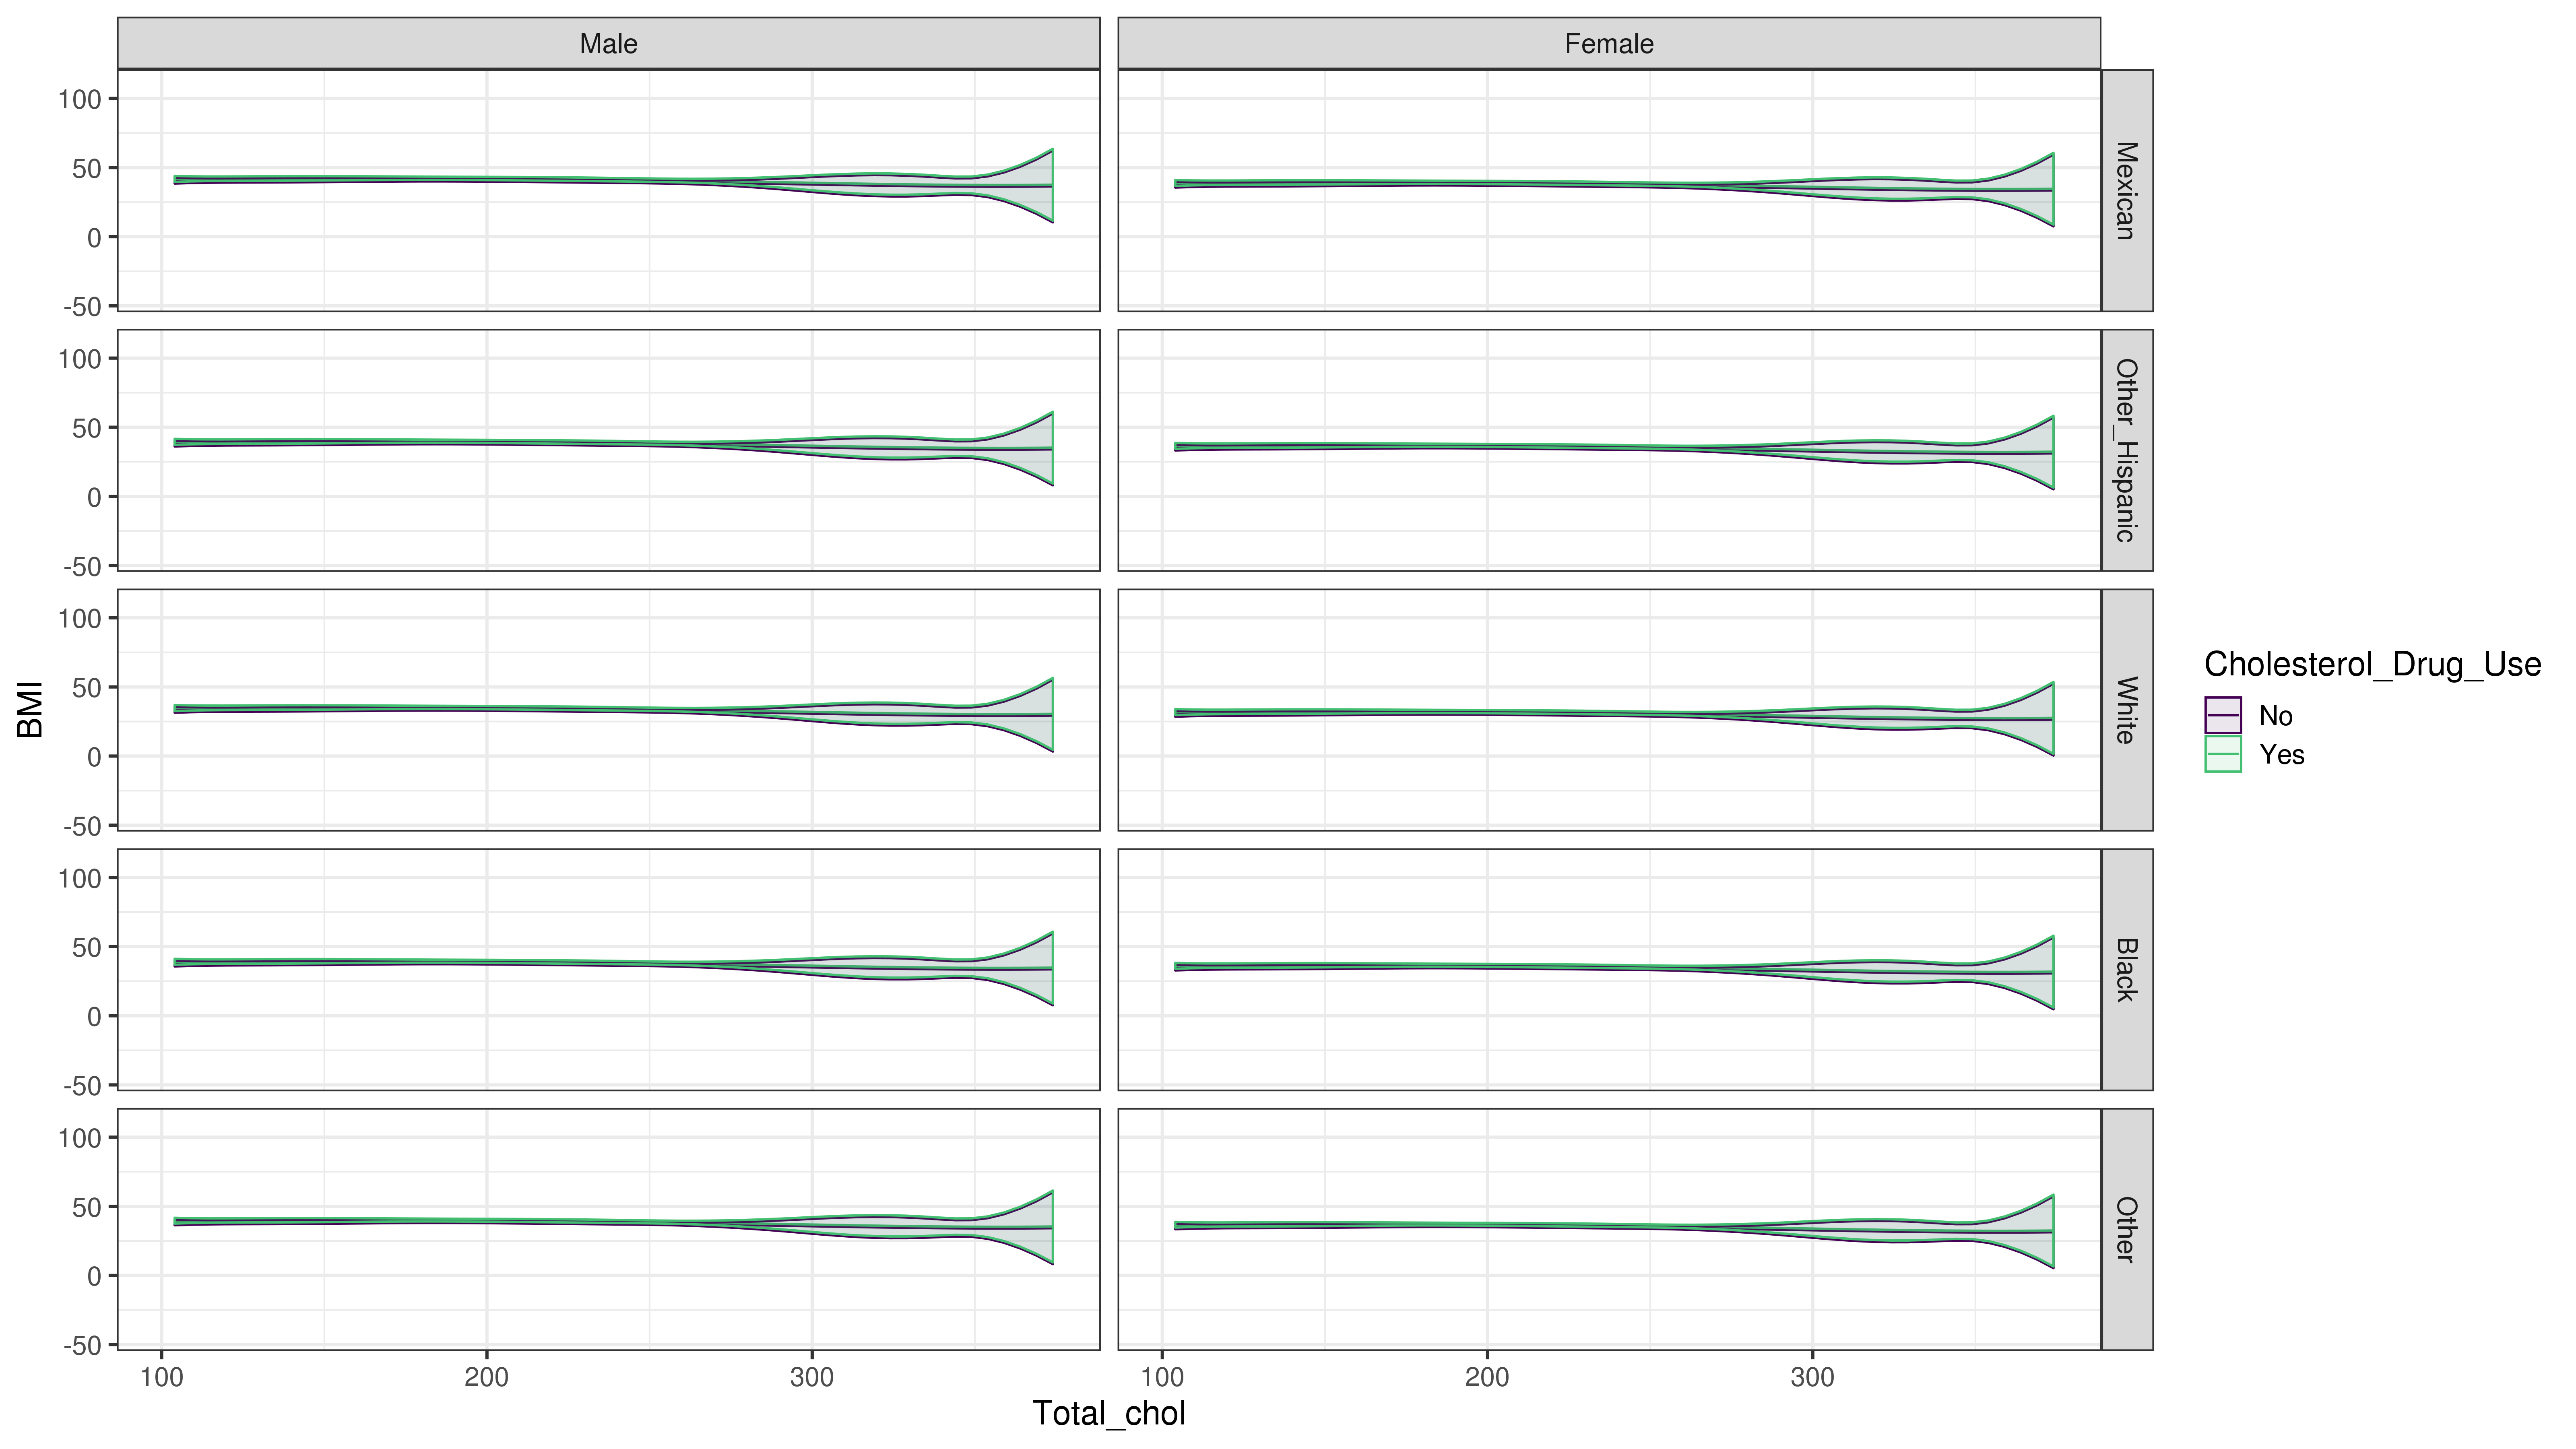
\includegraphics[width=0.8\linewidth]{/home/mabdulsa/BMI/images/TC_splin} 

}

\caption{ Illustration of a 90th quantile regression of the BMI. The cholesterol term modeled  using splines. }\label{fig:resu330}
\end{figure}

\section{Conclusion}

Multivariate quantile regression is used to study the effects of different risk factors on different BMI levels. our study shows that different risk factors for higher BMI have different effects on different quantiles. Moreover, predictors effect on BMI is subject to the methods used to represent it, which are quadratic modeling spline basis expansion. Quadratic term for the response to take a convex shape. This is different from spline basis expansions in which different polynomials have been used to model the predictors. Our results shows the turning point in the association between age and BMI is 30 years old. This is the age when people start to consider reducing weight. This trend is shown through the descriptive statistics and QR. However, quadratic modeling for the age is not able to detect this trend.

The effects of TC on the BMI is studied with respect to two ways for modeling TC. The turning point for patients to start reducing their BMI is when TC hit around 200 mg\(\setminus\)dL. However, if TC hits 350, the association become positive. This is a sign where patients are losing their control on their TC and BMI levels.

It is recommended to investigate why the effect estimates are varying across different BMI quantiles.

\newpage
\section{References}

\hypertarget{refs}{}
\leavevmode\hypertarget{ref-anderson1991}{}%
Anderson, Keaven M, Patricia M Odell, Peter WF Wilson, and William B Kannel. 1991. ``Cardiovascular Disease Risk Profiles.'' \emph{American Heart Journal} 121 (1): 293--98.

\leavevmode\hypertarget{ref-balkau2004prediction}{}%
Balkau, Beverley, Gang Hu, Qing Qiao, Jaakko Tuomilehto, Knut Borch-Johnsen, K Pyorala, DECODE Study Group, European Diabetes Epidemiology Group, and others. 2004. ``Prediction of the Risk of Cardiovascular Mortality Using a Score That Includes Glucose as a Risk Factor. The Decode Study.'' \emph{Diabetologia} 47 (12): 2118.

\leavevmode\hypertarget{ref-bann2020}{}%
Bann, David, Emla Fitzsimons, and William Johnson. 2020. ``Determinants of the Population Health Distribution: An Illustration Examining Body Mass Index.'' \emph{International Journal of Epidemiology} 49 (3): 731--37.

\leavevmode\hypertarget{ref-bruce2020}{}%
Bruce, Peter, Andrew Bruce, and Peter Gedeck. 2020. \emph{Practical Statistics for Data Scientists: 50+ Essential Concepts Using R and Python}. O'Reilly Media.

\leavevmode\hypertarget{ref-cade2003}{}%
Cade, Brian S, and Barry R Noon. 2003. ``A Gentle Introduction to Quantile Regression for Ecologists.'' \emph{Frontiers in Ecology and the Environment} 1 (8): 412--20.

\leavevmode\hypertarget{ref-calle1999body}{}%
Calle, Eugenia E, Michael J Thun, Jennifer M Petrelli, Carmen Rodriguez, and Clark W Heath Jr. 1999. ``Body-Mass Index and Mortality in a Prospective Cohort of Us Adults.'' \emph{New England Journal of Medicine} 341 (15): 1097--1105.

\leavevmode\hypertarget{ref-castro2016}{}%
Castro, M Regina, Gyorgy Simon, Stephen S Cha, Barbara P Yawn, L Joseph Melton, and Pedro J Caraballo. 2016. ``Statin Use, Diabetes Incidence and Overall Mortality in Normoglycemic and Impaired Fasting Glucose Patients.'' \emph{Journal of General Internal Medicine} 31 (5): 502--8.

\leavevmode\hypertarget{ref-chang2011}{}%
Chang, Jin-Biou, Nain-Feng Chu, Jhu-Ting Syu, An-Tsz Hsieh, and Yi-Ren Hung. 2011. ``Advanced Glycation End Products (Ages) in Relation to Atherosclerotic Lipid Profiles in Middle-Aged and Elderly Diabetic Patients.'' \emph{Lipids in Health and Disease} 10 (1): 228.

\leavevmode\hypertarget{ref-chen2005}{}%
Chen, Colin. 2005. ``Growth Charts of Body Mass Index (Bmi) with Quantile Regression.'' \emph{AMCS} 5: 114--20.

\leavevmode\hypertarget{ref-NHANES}{}%
Disease Control, Centers for, and Prevention (CDC). 2018. ``National Health and Nutrition Examination Survey Data (Nhanes.''

\leavevmode\hypertarget{ref-ferrieres2018}{}%
Ferrières, Jean, Dominik Lautsch, Anselm K Gitt, Gaetano De Ferrari, Hermann Toplak, Moses Elisaf, Heinz Drexel, et al. 2018. ``Body Mass Index Impacts the Choice of Lipid-Lowering Treatment with No Correlation to Blood Cholesterol--Findings from 52 916 Patients in the Dyslipidemia International Study (Dysis).'' \emph{Diabetes, Obesity and Metabolism} 20 (11): 2670--4.

\leavevmode\hypertarget{ref-flegal1999}{}%
Flegal, Katherine M. 1999. ``The Obesity Epidemic in Children and Adults: Current Evidence and Research Issues.'' \emph{Medicine and Science in Sports and Exercise} 31 (11 Suppl): S509--14.

\leavevmode\hypertarget{ref-hay2017gbd}{}%
Hay, Simon I, Sudha P Jayaraman, Alejandra G Contreras Manzano, Anoushka Millear, Laura Kemmer, Brent Bell, Juan Jesus Carrero, et al. 2017. ``GBD 2015 Risk Factors Collaborators. Global, Regional, and National Comparative Risk Assessment of 79 Behavioural, Environmental and Occupational, and Metabolic Risks or Clusters of Risks, 1990-2015: A Systematic Analysis for the Global Burden of Disease Study 2015 (Vol 388, Pg 1659, 2016).'' \emph{Lancet} 389 (10064): E1--E1.

\leavevmode\hypertarget{ref-katbody}{}%
Katzmarzyk, Peter T, Bruce A Reeder, Susan Elliott, Michel R Joffres, Punam Pahwa, Kim D Raine, Susan A Kirkland, and Gilles Paradis. 2012. ``Body Mass Index and Risk of Cardiovascular Disease, Cancer and All-Cause Mortality.'' \emph{Canadian Journal of Public Health} 103 (2): 147--51.

\leavevmode\hypertarget{ref-koenker2005}{}%
Koenker, Roger. 2005. ``Quantile Regression, Volume 38 of.'' \emph{Econometric Society Monographs}.

\leavevmode\hypertarget{ref-mc2020effects}{}%
Mc Auley, Mark Tomás. 2020. ``Effects of Obesity on Cholesterol Metabolism and Its Implications for Healthy Ageing.'' \emph{Nutrition Research Reviews} 33 (1): 121--33.

\leavevmode\hypertarget{ref-mozaffarian2015executive}{}%
Mozaffarian, Dariush, Emelia J Benjamin, Alan S Go, Donna K Arnett, Michael J Blaha, Mary Cushman, Sarah De Ferranti, et al. 2015. ``Executive Summary: Heart Disease and Stroke Statistics---2015 Update: A Report from the American Heart Association.'' \emph{Circulation} 131 (4): 434--41.

\leavevmode\hypertarget{ref-nuttall2015body}{}%
Nuttall, Frank Q. 2015. ``Body Mass Index: Obesity, Bmi, and Health: A Critical Review.'' \emph{Nutrition Today} 50 (3): 117.

\leavevmode\hypertarget{ref-pandya2015}{}%
Pandya, Ankur, Stephen Sy, Sylvia Cho, Milton C Weinstein, and Thomas A Gaziano. 2015. ``Cost-Effectiveness of 10-Year Risk Thresholds for Initiation of Statin Therapy for Primary Prevention of Cardiovascular Disease.'' \emph{Jama} 314 (2): 142--50.

\leavevmode\hypertarget{ref-ridker2012}{}%
Ridker, Paul M, Aruna Pradhan, Jean G MacFadyen, Peter Libby, and Robert J Glynn. 2012. ``Cardiovascular Benefits and Diabetes Risks of Statin Therapy in Primary Prevention: An Analysis from the Jupiter Trial.'' \emph{The Lancet} 380 (9841): 565--71.

\leavevmode\hypertarget{ref-sugiyama2014}{}%
Sugiyama, Takehiro, Yusuke Tsugawa, Chi-Hong Tseng, Yasuki Kobayashi, and Martin F Shapiro. 2014. ``Different Time Trends of Caloric and Fat Intake Between Statin Users and Nonusers Among Us Adults: Gluttony in the Time of Statins?'' \emph{JAMA Internal Medicine} 174 (7): 1038--45.

\leavevmode\hypertarget{ref-tsaousis2014}{}%
Tsaousis, Konstantinos T. 2014. ``Blood Glucose and Cholesterol Concentrations in a Mediterranean Rural Population of Andros Island, Greece.'' \emph{International Journal of Preventive Medicine} 5 (11): 1464.

\leavevmode\hypertarget{ref-van2012estimating}{}%
Van de Kassteele, Jan, RT Hoogenveen, PM Engelfriet, PHM Van Baal, and HC Boshuizen. 2012. ``Estimating Net Transition Probabilities from Cross-Sectional Data with Application to Risk Factors in Chronic Disease Modeling.'' \emph{Statistics in Medicine} 31 (6): 533--43.

\leavevmode\hypertarget{ref-yusuf2016}{}%
Yusuf, Salim, Jackie Bosch, Gilles Dagenais, Jun Zhu, Denis Xavier, Lisheng Liu, Prem Pais, et al. 2016. ``Cholesterol Lowering in Intermediate-Risk Persons Without Cardiovascular Disease.'' \emph{New England Journal of Medicine} 374 (21): 2021--31.

\leavevmode\hypertarget{ref-yusuf2004effect}{}%
Yusuf, Salim, Steven Hawken, Stephanie Ôunpuu, Tony Dans, Alvaro Avezum, Fernando Lanas, Matthew McQueen, et al. 2004. ``Effect of Potentially Modifiable Risk Factors Associated with Myocardial Infarction in 52 Countries (the Interheart Study): Case-Control Study.'' \emph{The Lancet} 364 (9438): 937--52.

\end{document}
